\newcommand{\autor}{Pedro Pozuelo Rodríguez}
\newcommand{\titulo}{Reverse Proxy con capacidades de Firewall de aplicación web y aceleración TLS}
\newcommand{\profesor}{Ana del Valle Corrales Paredes}
\newcommand{\PFGID}{Pendiente}
\newcommand{\fechaversion}{\today}

\newcommand{\pfg}[1]{\par \textbf{{\color{blue} GUIDE: }{#1}}}
\newcommand{\wip}{\par {\color{red} WIP}}

% \documentclass[a4paper,11pt,spanish]{article}
\documentclass[a4paper,11pt,spanish]{report}

\usepackage{amsmath, amssymb, latexsym}
\usepackage[margin=2.5cm]{geometry}
\usepackage{xltxtra}

% Highlight where is the paragraph overfull \hbox error (adding a black bar where a line is too wide)
\overfullrule=2cm

% Allows us to wrap underlined text
\usepackage{soul}

% \usepackage[spanish]{babel} % Se ha sustituido por Polyglossia
\usepackage{polyglossia}
  \setmainlanguage{spanish}
  \setmainfont[Mapping=tex-text]{Linux Libertine O}
  \defaultfontfeatures{Ligatures=TeX}

% \usepackage{titlesec}
%  \titleformat{\chapter}[display]
%    {\normalfont\bfseries}{}{0pt}{\Huge}

\usepackage{ifpdf}
\usepackage{moreverb}
\usepackage{multicol}
\usepackage{epsfig}
\usepackage{tikz}
\usepackage{color}
\usepackage{colortbl}
\usepackage{enumerate}
\usepackage{titlesec}
\usepackage{appendix}
\addto\captionsspanish{%
  \appendixtitleon
  \renewcommand{\appendixname}{Anexo}
  \renewcommand\appendixpagename{Anexos} }
\usepackage{msc}                % Draw Message Sequence Charts
\usepackage{scalefnt}           % Rescale fonts to arbitrary sizes
\usepackage{xurl}
\usepackage[pdfencoding=unicode,
            unicode=true,
            bookmarks=true,
            colorlinks=true, 
            pdfstartview=FitH, 
            linkcolor=blue, 
            citecolor=blue, 
            breaklinks=true,
            bookmarksopen=true,
            urlcolor=blue]
            {hyperref}
\usepackage[all]{hypcap}
\usepackage[color={0 0 1}]{attachfile2}
\usepackage{listings}
\usepackage[all]{xy}            % Paquete para dibujar diagramas (\xymatrix)
\usepackage{changepage}         % Útil para modificar márgenes en mitad del documento
\usepackage[shortlabels]{enumitem}
\usepackage{tabularx}
\usepackage{tabulary}
\usepackage{mathtools}
\usepackage{pdflscape}
\usepackage[autostyle]{csquotes} 
\usepackage{subcaption}

\selectlanguage{spanish}

%% Figures within a column...
\makeatletter
\newenvironment{tablehere}
{\def\@captype{table}}
{}
\newenvironment{figurehere}
{\def\@captype{figure}}
{}
\makeatother

\oddsidemargin 0in
\textwidth 6.25in

\title{\titulo{}}
\author{\autor{}}
\date{\today}

%% Información para el PDF que se genera.
\ifpdf
  \pdfinfo{
    /Author (\autor{})
    /title{\titulo{}}
  }
\fi

% Gestión de la bibliografía.
\usepackage[
  backend=biber,
  style=numeric,
  sorting=none
]{biblatex}

% Create glossary and definitions
\usepackage[acronyms,toc]{glossaries}

%% Información para los ficheros adjuntos.
\attachfilesetup{author=\autor{}}

%% Redefinimos el aspecto del título de las secciones
%\renewcommand{\thesection}{Problema \arabic {section}.}

%% Redefinimos el tamaño de la fuente en \section y \subsection
%\titleformat{\section}{\large\bfseries\em}{Parte \thesection.}{1em}{}
%\titleformat{\subsection}{\normalsize\bfseries}{Parte \thesubsection.}{1em}{}
%\titleformat{\subsubsection}{\normalsize\bfseries}{Parte \thesubsubsection.}{1em}{}

%% Definimos el tamaño de la fuente para verbatim en small
\makeatletter
  \g@addto@macro\@verbatim\small
\makeatother 

%% Indicamos un interlineado de 1.5
% \renewcommand*{\baselinestretch}{1.5}

%% Aumentamos el espacio de nuevo párrafo
\parskip=2mm

%% Propiedades del código fuente para todo el documento
\definecolor{dkgreen}{rgb}{0,0.6,0}
\definecolor{gray}{rgb}{0.5,0.5,0.5}
\definecolor{mauve}{rgb}{0.58,0,0.82}
\lstset{numbers=left,
        basicstyle=\scriptsize,
        frame=single,
        breaklines=true,
        %title=\lstname,
        language=bash,
        keywordstyle=\color{blue},
        commentstyle=\color{dkgreen},
        stringstyle=\color{mauve},
				showstringspaces=false,
        extendedchars=true,
        %texcl,
        tabsize=2}
\def\inline{\lstinline[language=bash,
		basicstyle=\normalsize,
		keywordstyle=\color{blue},
		commentstyle=\color{dkgreen},
		stringstyle=\color{mauve},
		extendedchars=true,
		showstringspaces=false,
    texcl]}

\usepackage{dirtytalk}

\newcommand*\greenarrow{%
  \color{green!80!black}{$\Uparrow$}
}

\newcommand*\redarrow{%
  \color{red!80!black}{$\Downarrow$}
}

\newcommand*\yellowarrow{%
  \color{yellow!80!black}{$\Rightarrow$}
}


% \hyphenation{pri-va-ti-vas}
\hyphenation{in-fra-es-truc-tu-ra}
\hyphenation{Cloud-Fla-re}
\hyphenation{ge-ne-ren}
\hyphenation{li-cen-cia-mien-to}
\hyphenation{pri-va-ti-vo}
\hyphenation{pro-ce-de}
\hyphenation{pla-ta-for-ma}
\hyphenation{me-jo-rar}
\hyphenation{ad-qui-rien-do}
\hyphenation{de-di-ca-das}
\hyphenation{pro-ve-e-do-res}
\hyphenation{de-pen-dien-do}
\hyphenation{in-me-dia-ta-men-te}
\hyphenation{a-pli-ca-ción}



\addbibresource{bib/Referencias.bib}

% Change the path accordingly
\def \codePath {../../CircumCaetera}

% Create a glossary for terms and definitions
\makeglossaries
\newacronym{gcd}{GCD}{Greatest Common Divisor}
\newacronym{lcm}{LCM}{Least Common Multiple}
\newacronym{waf}{WAF}{Web Application Firewall}
\newacronym{saas}{SaaS}{Software as a Service}
\newacronym{cdn}{CDN}{Content Delivery Network}
\newacronym{dos}{DoS}{Denial-of-service}
\newacronym{SNI}{SNI}{Server Name Indication\cite{TLSSNI}}
\newacronym{ev}{EV}{Extended Validation}
\newacronym{rbac}{RBAC}{role-based access control}
\newacronym{dbf}{DBF}{Database Firewall}
\newacronym{rgdp}{RGDP}{Reglamento General de Protección de Datos}
\newacronym{pcidss}{PCI DSS}{Payment Card Industry Data Security Standard}
\newacronym{xss}{XSS}{Cross-site scripting\cite[Artículo en OWASP]{owaspxss}}
\newacronym{sqli}{SQLi}{SQL injection\cite[Artículo en OWASP]{owaspsqli}}
\newacronym{poc}{PoC}{Proof of concept}
\newacronym{gpl}{GPL}{GNU General Public License\cite[Licencia GPL]{gpl}}
\newacronym{lgpl}{LGPL}{GNU Lesser General Public License\cite[Licencia LGPL]{lgpl}}
\newacronym{siem}{SIEM}{Security information and event management}
\newacronym{ca}{CA}{Certification Authority}


\newglossaryentry{throughput}
{
    name=Throughput,
    description={La tasa de transferencia efectiva (en inglés throughput) es el volumen de trabajo o de información neto que fluye a través de
    un sistema, como puede ser una red de computadoras.}~\cite[Wikipedia]{wikithroughput}
}

\newglossaryentry{CA}
{
    name=CA,
    description={En criptografía, las expresiones autoridad de certificación, o certificadora, o certificante, o las siglas AC o CA (por la
    denominación en idioma inglés Certification Authority), señalan a una entidad de confianza, responsable de emitir y revocar los certificados,
    utilizando en ellos la firma electrónica, para lo cual se emplea la criptografía de clave pública.}~\cite[Wikipedia]{CA}
}

\newglossaryentry{Atacante}
{
    name=Atacante,
    description={El atacante es un individuo u organización que intenta obtener el control de un sistema informático para utilizarlo con fines
    maliciosos, robo de información o de hacer daño a su objetivo.}~\cite[Wikipedia]{Atacante}
}



\begin{document}

%%%%%%%%%%%%%%%%%%%%%%%%%%%%%%%%%%%%%%%%%%%%%%%%%%%%%%%%%%%%%%%%%%%%%%%%%%%%%%%%%%%%%%%%%%%%%%%%%%%%%%%%%
%%%%%%%%%%%%%%%%%%%%%%%%%%%%%%%%%%%%%%%%% Parámetros de portada %%%%%%%%%%%%%%%%%%%%%%%%%%%%%%%%%%%%%%%%%
%%%%%%%%%%%%%%%%%%%%%%%%%%%%%%%%%%%%%%%%%%%%%%%%%%%%%%%%%%%%%%%%%%%%%%%%%%%%%%%%%%%%%%%%%%%%%%%%%%%%%%%%%
%%%%%%%%%%%%%%%%% Utilizamos una portada externa %%%%%%%%%%%%%%%%%%%%%%%%%%%%%%%%%%%%%%%%%%%%%%%%%%%%%%%%
%  \pagenumbering{roman}
%  \thispagestyle{empty}
%  \newgeometry{margin=0cm,top=2cm}
%  \begin{center}
%    \includegraphics[width=0.9\textwidth]{Portada.pdf}
%  \end{center}
%  \restoregeometry
% 
%%%%%%%%%%%%%%%%%%%%%%%%%%%%%%%%%%%%% Creamos un título dinámicamente %%%%%%%%%%%%%%%%%%%%%%%%%%%%%%%%%%%
% \maketitle


 
\begin{titlepage}
    \begin{center}
        
\includegraphics[width=0.4\textwidth]{fig/universidad_logo}
        \vspace*{2cm}
 
        \Huge
        \textbf{Universidad Europea\\Proyecto de Fin de Grado}
 
        \vspace{3cm}
        \LARGE
        \textbf{\titulo}
 
        \vfill
 
 
    \end{center}

    \Large
    \begin{tabular}{ll}
      Alumno:			    & \autor\\
      Directora:		  & \profesor\\
      Titulación:			& Grado en Ingeniería Informática\\
      Fecha:          & \fechaversion
    \end{tabular}
\end{titlepage}
%
%%%%%%%%%%%%%%%%%%%%%%%%%%%%%%%%%%%%%%%%%%%%%%%%%%%%%%%%%%%%%%%%%%%%%%%%%%%%%%%%%%%%%%%%%%%%%%%%%%%%%%%%%
%%%%%%%%%%%%%%%%%%%%%%%%%%%%%%%%%%%%%%%%% Parámetros de índice %%%%%%%%%%%%%%%%%%%%%%%%%%%%%%%%%%%%%%%%%%
%%%%%%%%%%%%%%%%%%%%%%%%%%%%%%%%%%%%%%%%%%%%%%%%%%%%%%%%%%%%%%%%%%%%%%%%%%%%%%%%%%%%%%%%%%%%%%%%%%%%%%%%%
%%%%%%%%%%%%%%%%%%%%%%%%%%%%%%%%%%%%%%%%%%% Portada externa %%%%%%%%%%%%%%%%%%%%%%%%%%%%%%%%%%%%%%%%%%%%%
%  \thispagestyle{empty}
%  \newpage
%  \pagenumbering{arabic}
% 
%%%%%%%%%%%%%%%%%%%%%%%%%%%%%%%%%%%%%%% Índice del documento %%%%%%%%%%%%%%%%%%%%%%%%%%%%%%%%%%%%%%%%%%%%
% \clearpage
\tableofcontents
% \listoffigures
%%%%%%%%%%%%%%%%%%%%%%%%%%%%%%%%%% Índice del documento (pequeño)  %%%%%%%%%%%%%%%%%%%%%%%%%%%%%%%%%%%%%%
% {\small\tableofcontents}

%%%%%%%%%%%%%%%%%%%%%%%%%%%%%%%%%%%%% Índice de código fuente %%%%%%%%%%%%%%%%%%%%%%%%%%%%%%%%%%%%%%%%%%%
% \lstlistoflistings
% \clearpage
%%%%%%%%%%%%%%%%%%%%%%%%%%%%%%%%%%%%%%%%%%%%%%%%%%%%%%%%%%%%%%%%%%%%%%%%%%%%%%%%%%%%%%%%%%%%%%%%%%%%%%%%%



\chapter{Introducción}
\par En los últimos años, la mayoría de los ataques en Internet se realizan contra aplicaciones web, con lo que es cada vez más importante
contar con una solución que sea capaz de analizar el tráfico web y proteger dichas aplicaciones.
\par Desgraciadamente, no existe una aplicación completamente segura tal como afirma el adagio:

\say{La seguridad 100\% no existe.}

\par Con este punto de partida, y teniendo en cuenta el uso masivo que las aplicaciones hacen del Protocolo de transferencia de hipertexto (en adelante \acrshort{http}, de sus siglas en inglés\acrlong{http}) y del
Protocolo seguro de transferencia de hipertexto (en adelante \acrshort{https}, de sus siglas en inglés \acrlong{https}), es inmediato identificar porqué la mayoría de los ataques actuales se realizan contra aplicaciones publicadas a través de
estos protocolos.

\par Para protegerlas existen múltiples mecanismos de seguridad, desde herramientas que monitorizan el uso indebido de datos como el Software de prevención de pérdida de datos (en
adelante \acrshort{dlp}, de sus siglas en inglés \acrlong{dlp}), herramientas de red como son el firewall tradicional o herramientas más dirigidas como son los firewall de
aplicación web (en adelante \acrshort{waf}, de sus siglas en inglés, \acrlong{waf}).

\par En entornos con una gran infraestructura, que generen una facturación importante o con un alto riesgo, es habitual que se desplieguen las herramientas mencionadas y muchas otras, incluso herramientas redundantes siguiendo el principio de
\gls{DefensaProfundidad},  el cual aboga por desplegar múltiples sistemas de protección con el fin de que si uno falla otro pueda detener el ataque.
\par Pero, en entornos en los que los recursos son más limitados, no es viable desplegar todos los controles de seguridad que serían deseables. Por recursos no sólo se entiende
económicamente limitados como para invertir en tecnologías, si no también por personas con el tiempo, el conocimiento y la experiencia como para desplegar y mantenerlas.
\par En estos entornos es habitual que los controles de seguridad se limiten a un firewall de red o, si se dispone de algo más de presupuesto, un sistema de Gestión Unificada de
Amenazas (más conocido como \acrshort{utm}, de sus siglas en inglés\acrlong{utm}~\cite{wiki:utm}).
\par Estas soluciones, desgraciadamente, no son capaces de ofrecer una protección adecuada contra ataques en capa de aplicación. Por ejemplo, los firewall tradicionales son
capaces de analizar el tráfico de red en capa 3 del modelo TCP/IP (equivalente a las capas 3 y 4 del {\em modelo OSI\cite{osi}}). Esto implica que , cuando se publica un servicio web,
dichos firewalls permitirán todo el tráfico dirigido a estos servicios, con independencia de que se trate de una petición legítima, una petición incorrectamente formada o un ataque.
\par Para proteger estos servicios web adecuadamente es necesario disponer de tecnologías que entiendan analicen el tráfico en la capa de aplicación siguiendo la lógica propia del servicio a proteger, como los mencionados
WAF.

\par Otro aspecto que se debe tener en cuenta consiste en la migración constante que se está produciendo de forma generalizada de tráfico sin cifrar - también conocido como en texto plano - a tráfico cifrado HTTPS en el que se
encapsula el tráfico HTTP en un canal SSL/TLS. Históricamente se utilizaban múltiples herramientas perimetrales como son los sistema de detección de intrusiones (en adelante \acrshort{nids}, de sus siglas en inglés \acrlong{nids}) o los
mencionados firewalls. Desgraciadamente estas herramientas tradicionalmente no participan en la negociación SSL/TLS, por lo que no son capaces de descifrar el tráfico y no pueden analizar el contenido de las peticiones o sus respuestas. Estas
herramientas son, por lo tanto, cada vez menos efectivas a la hora de detectar y bloquear amenazas, pues carecen de la visibilidad adecuada en un gran porcentaje del tráfico.
\par Por último, se debe considerar otro cambio significativo que se está produciendo en estos últimos años: Cada vez es más habitual desplegar las aplicaciones en ~\gls{cloud} (o cloud, se utilizarán ambos términos indistintamente
debido a su uso extendido). En estos entornos se diluyen los conceptos de red perimetral o segmentación de red y es más complejo desplegar controles de seguridad perimetrales como los mencionados firewalls, NIDS o UTM. En estos entornos muchos
de los componentes de la infraestructura son transparentes para el cliente y no es posible desplegar mecanismos en estas capas.
\par A modo de referencia en la imagen {~\hyperref[fig:Responsabilidadescloud]{Responsabilidades compartidas en el cloud}} (fuente MR Informática~\cite{Responsabilidadescloud}) vemos como los únicos elementos sobre los que se mantiene el
control en los distintos modelos del cloud son la capa de aplicación y los datos (con la excepción del modelo de Software como un Servicio, en adelante \acrshort{saas}, de sus siglas en inglés \acrlong{saas}).
\begin{center}
  \label{fig:Responsabilidadescloud}
  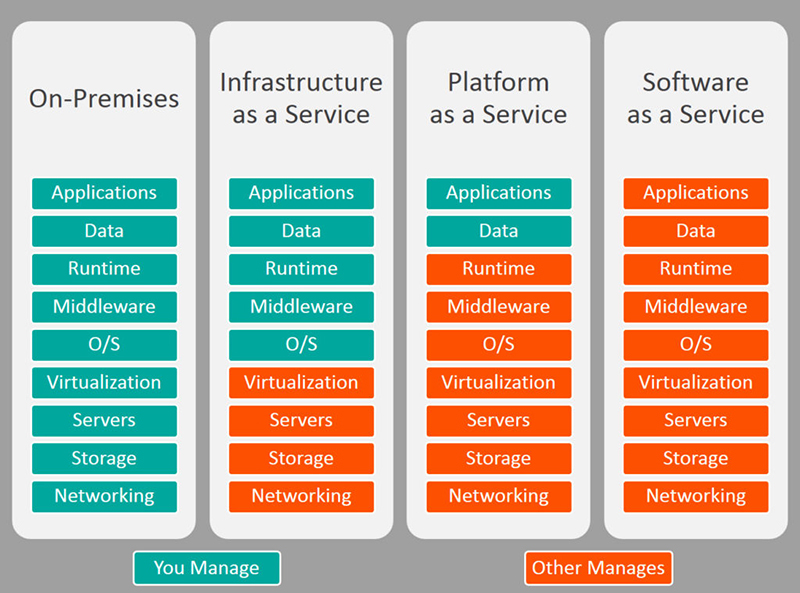
\includegraphics[width=0.7\textwidth]{fig/Responsabilidadescloud}
\end{center}

\par Es por lo tanto, cada vez más importante contar con herramientas que sean capaces de descifrar y analizar el tráfico HTTPS y, según se verá con más detalle en la sección de ~\nameref{subsec:estadoarte}, estas soluciones implican o bien un
desembolso económico significativo en el caso de las soluciones privativas o bien se despliegan como módulos de la propia aplicación web en las soluciones de {\em software libre\cite{softwarelibre}}.
\par En este segundo grupo las soluciones requieren un ejercicio de integración con las aplicaciones web y consumen recursos del servidor que pueden impactar en el rendimiento. Adicionalmente, para la implementación y configuración adecuada de
estos módulos se requiere de una persona con un conocimiento profundo de la seguridad de aplicaciones web que se mantenga informado de las últimas novedades del sector y que administre y actualice el entorno según se detectan nuevos ataques y
mecanismos paliativos.  Debido a estos factores y la complejidad que el WAF añade a la plataforma web, es habitual que cuando una plataforma web requiere de una actualización importante o una migración de tecnologías, el modulo de WAF se
desactive o elimine completamente.

\par Como respuesta a esta necesidad surge el presente proyecto, cuyo objetivo es construir una solución de software libre con capacidades de WAF, aceleración SSL/TLS, fácilmente desplegable y que minimice el esfuerzo y el impacto que dicha
solución tiene sobre la plataforma web actual o futura.


\chapter{Estado del arte}
\label{subsec:estadoarte}
\par Tal como se ha comentado en el capítulo anterior, un elemento clave para proteger las aplicaciones web es el WAF.

\par En primer lugar se ha procedido a realizar una análisis comparativo de las diferentes soluciones WAF disponibles en el mercado. Para ello, se ha utilizado el documento de buenas prácticas de OWASP\cite{owaspbestpractices} como referencia.
\par forma específica, el criterio seguido es que la solución debe ser capaz de proteger la plataforma web implementando una mayoría de los controles de seguridad (referenciados como {\em Countermeasure} en la página de OWASP\cite[apartado A3.2]{owaspbestpractices}).

\par Dentro de las soluciones disponibles, podemos distinguir principalmente entre soluciones privativas y soluciones de software libre. Este
criterio no se circunscribe exclusivamente al modelo de licencias si no que está íntimamente ligado al coste asociado tal como veremos.

\section{Soluciones WAF privativas}
\par Las soluciones de WAF privativas se caracterizan por emplear un modelo de {\em licenciamiento privativo\cite{privativo}}. Se trata de
soluciones con un elevado coste y con la imposibilidad de acceder al código o modificarlo. Así mismo, ofrecen una serie de funcionalidades
adicionales y una mayor capacidad de procesamiento.
\par Existen dos arquitecturas principales en este tipo de WAF:
\par Por un lado tenemos modelos WAF desplegados en las instalaciones del fabricante y gestionados por él. Este tipo de soluciones suelen estás
alojadas en el Cloud (en el modelo de distribución de software conocido como {\em software como servicio} (en adelante \acrshort{saas}, de sus
siglas en inglés, \acrlong{saas}).
\par En segundo lugar, tenemos WAF de tipo appliance o máquina virtual. Se trata de máquinas dedicadas en las que el software requiere de una
máquina específica proporcionada por el fabricante. Si bien hardware y software se adquieren conjuntamente, es posible acceder a nuevas
funcionalidades adquiriendo nuevas licencias.

\subsection{Soluciones WAF SaaS}
\par Dentro de las soluciones WAF SaaS, destacan y se han analizado {\em Cloud Web Application Firewall} \cite{cloudflarewaf} de Cloudflare\cite{cloudflare} ({\em Cloudflare} en adelante), {\em Kona WAF\cite{kona}} de {\em Akamai\cite{akamai}} e {\em Incapsula\cite{Incapsula}}.
\par Habitualmente, estos proveedores no se limitan a ofrecer servicios WAF, pues por su infraestructura permite añadir funcionalidades adicionales como son las siguientes.
\begin{itemize}
  \item Red de distribución de contenidos (en adelante \acrshort{cdn}, de sus siglas en inglés, \acrlong{cdn}).
  \item Protección contra ataques de denegación de servicio (en adelante \acrshort{dos}, de sus siglas en inglés, \acrlong{dos}) en capa de
    aplicación.
  \item Habilitar el caché de contenido estático.
  \item Suscripción a listas de reputación de IP, dominios o URL.
  \item Bloqueo de bots maliciosos.
  \item Sistema de creación de informes.
\end{itemize}
\par De hecho, la funcionalidad CDN es el servicio mínimo que se puede contratar a Akamai y Cloudflare; pues es su nicho mercado y su producto
principal, siendo el servicio WAF una funcionalidad que ofrecen a sus cliente para dar un valor añadido. Incapsula, por el contrario, proviene
de soluciones WAF tipo appliance y su modelo de negocio está más enfocado a estos servicios.
\par Uno de las principales características que comparten estos proveedores es el modelo de negocio. En todos los casos el coste está asociado
al volumen de tráfico que se genere, ya sea en caudal de datos (en adelante \gls{throughput}), como es el caso de Incapsula, o por volumen mensual de datos en el caso de Akamai y Cloudflare.

\subsubsection{Modo de licenciamiento y coste}
\label{subsec:wafsaaslic}
\par En la mayoría de las soluciones no existe un precio oficial de mercado proporcionado por los proveedores. En estos casos se ha optado por
incluir referencias externas con el fin de disponer información del coste aproximado de estas soluciones.
\par A modo de referencia, se puede consultar los precios de Akamai y Cloudflare en la {~\hyperref[tab:precioscdn]{tabla de precios CDN}}.
Estos precios se corresponden con sus servicios de CDN y podrá ser superior si se añaden funcionalidades como WAF. Adicionalmente, se debe
tener en cuenta que se trata de precios estimativos proporcionados por terceros, pues en el caso de Akamai la lista de precios no es pública y
ofrecen un coste ajustado a cada cliente.
\begin{table}[h!]
  \centering
  \label{tab:precioscdn}
  \begin{tabular}{rrr}
     &
    \multicolumn{1}{c}{\textbf{Akamai CDN}} &
    \multicolumn{1}{c}{\textbf{CloudFlare CDN}} \\
    \hline \hline
    6 TB plan   & 900  USD al mes aprox.  & 750   USD al mes aprox. \\
    \hline
    25 TB plan  & 2800 USD al mes aprox.  & 2800  USD al mes aprox. \\
    \hline
    50 TB plan  & 5500 USD al mes aprox.  & 5000+ USD al mes aprox. \\
    \hline
    100 TB plan & 8000 USD al mes aprox.  & 5000+ USD al mes aprox. \\
    \hline
  \end{tabular}
  \caption{Precios de CDN\cite{cdnprices} (consultado en abril de 2019)}
\end{table}

\par En el caso de Incapsula, su solución más económica - el plan {\em PRO} -  tiene un coste de 59 USD por web al mes\cite{incapsulaprices}.
Dicha solución soporta SSL de manera limitada y es necesario contratar un plan superior en caso de que se requiera dar servicio a clientes que
no soporten la extensión TLS \acrshort{SNI} o se requieran certificados con validación extendida (en adelante \acrshort{ev}, de sus siglas en
inglés, \acrlong{ev}). En esta situación habría que contratar el plan {\em business} que tiene un coste de 299 USD por web al
mes\cite{incapsulaprices}.

\subsubsection{Implementación y operación}
\par Independientemente de la solución, grosso modo estos son los pasos a realizar para implantar este tipo de soluciones:
\begin{enumerate}
  \item Cambio en la gestión de certificados SSL.
    \par Dado que la mayoría de las aplicaciones web deben soportar SSL, es necesario generar nuevos certificados para que el proveedor pueda
    publicar los servicios web de manera confiable. En la mayoría de los casos el fabricante será responsable del mantenimiento y la operación
    de dichos certificados.
  \item Preparación de un entorno de pruebas - {\em staging} - en el que se puedan probar las aplicaciones web de manera interna sin impactar
    a los clientes. Para ello, habitualmente, se redireccionan los dominios a probar en el fichero {\em hosts} de la máquina cliente.
  \item Cambio del direccionamiento DNS.
    \par Una ya se ha validado que la solución web y el WAF funcionan adecuadamente, se procede a cambiar el direccionamiento ofrecido a nivel
    DNS para que los clientes se conecten a la plataforma WAF en lugar de a la aplicación web.
\end{enumerate}

\par La operación de estas plataformas es realizada por el proveedor, por lo que como clientes no necesitamos disponer del conocimiento o el
tiempo necesario para mantener o actualizar la plataforma WAF.

\subsubsection{Ventajas}
\par Una de las principales ventajas que tiene este tipo de soluciones consiste en su independencia respecto a la infraestructura de la
aplicación web.
\par Esta independencia nos permite realizar cambios en cualquier de las soluciones - WAF o plataforma Web - sin que afecte a la otra. Ya sean
cambios en la operación diaria, migraciones de software o rediseño de la arquitectura.
\par La mencionada independencia no se limita a independencia tecnológica; el hecho de que el WAF y la plataforma web sean completamente
independientes también permite asignar roles independientes a cada entorno, lo cual permite implementar seguridad basada en roles (en adelante
\acrshort{rbac}, de sus siglas en inglés, \acrlong{rbac}). Esto no sólo nos permite mejorar la seguridad del entorno, si no que además evita
que el desarrollador web o el administrador de la plataforma web tenga que conocer en detalle la configuración del WAF y viceversa.

\par Por otro lado, este tipo de soluciones son las muy sencillas de implementar, tal como se ha visto en la sección anterior.
\par Otra ventaja radica en la aplicación de nuevas reglas de seguridad de forma transparente para el cliente. No necesitaremos dar seguimiento
a las últimas vulnerabilidades web que se publican o idear qué reglas o firmas son necesarias, pues el proveedor se hará cargo de su
implementación y mantenimiento.
\par Las soluciones WAF SaaS también nos permiten contratar diversas modalidades de soporte que garanticen respuesta 24/7 en caso de que se
produzca un incidente con el servicio.
\par Por último, nos podemos beneficiar de las funcionalidades adicionales ya mencionadas para mejorar el estado de la seguridad de nuestra
plataforma o mejorar la experiencia del usuario.


\subsubsection{Desventajas}
\par Una de las principales desventajas radica en el coste económico. Este tipo de soluciones tienen un elevado coste. Esto implica que este tipo de WAF sólo son viables económicamente en portales que generen un beneficio económico importante o aquellos en los que la empresa/entidad responsable de la aplicación pueda asumir su inversión.
\par Aunque este tipo de soluciones disponen de modalidades relativamente económicas (ver ~\nameref{subsec:wafsaaslic}), lo cierto es que estas soluciones
están muy limitadas y es necesario contratar funcionalidades adicionales en la mayoría de los casos. Es un modelo económico muy dirigido a las
ofertas personalizadas y suele ser habitual requerir el modelo de licenciamiento {\em Enterprise} junto con ciertas licencias adicionales, lo
cual encarece todavía más el servicio.
\par En cualquier caso, este tipo de soluciones no están al alcance de pequeñas o medianas empresas o de particulares.

\par Otra desventaja que tienen este tipo de soluciones consiste en la pocas posibilidades que tenemos de personalizar las reglas o las firmas
a nuestras necesidades. La arquitectura de este tipo de plataformas SaaS consiste en que múltiples clientes comparten la misma plataforma, para
lo cual el proveedor requiere mantener un sistema homogéneo para todos los clientes y esto evita que se pueda personalizar el WAF según
nuestras necesidades. A modo de ejemplo, en los servicios estándar de este tipo de soluciones no podremos configurar reglas para filtrar las
cabeceras HTTP o los parámetros de tipo query en las URL si nuestra aplicación utilizada {\em Path Parameters} o {\em URL Routing}, lo que
dejaría expuesta la aplicación web a ataques de inyección de código.


\subsection{Soluciones WAF tipo Appliance}
\par Otra modalidad de soluciones WAF son los de tipo appliance. Dentro de las opciones disponibles en el mercado se han analizado {\em Imperva
WAF Gateway\cite{imperva}} ({\em Imperva} en adelante) y {\em Fortiweb\cite{fortiweb}} de la empresa {\em Fortinet\cite{fortinet}}.
\par El modelo de negocio tradicional consiste en adquirir máquina física junto con un paquete de licencias, aunque en los últimos años se han
incorporado soluciones virtuales en los catálogos de los principales proveedores de Cloud.
\par Al igual que sucede con las soluciones SaaS, los proveedores de este tipo de WAF también incluyen mecanismos de seguridad adicionales que
no son propiamente funcionalidades WAF. Si bien estas funcionalidades dependen en gran medida del proveedor, a continuación se enumeran algunas
de las más interesantes:
\begin{itemize}
  \item Crear perfiles de las aplicaciones web y filtrar las peticiones web en función de los parámetros permitidos.
  \item Parcheo virtual de vulnerabilidades mediante la integración del WAF con programas de escaneo de vulnerabilidades.
  \item Suscripción a listas de reputación de IP, dominios o URL.
  \item Aceleración TLS.
    \par Dado que el dispositivo suele estar en la misma red que la aplicación web, es posible que el WAF realice el descifrado del tráfico
    SSL/TLS y envíe el tráfico sin cifrar a la aplicación web, lo que permite liberar los recursos asignados al cifrado y descifrado en la
    aplicación web.
  \item Bloqueo de bots maliciosos.
  \item Sistema de creación de informes.
  \item Antivirus.
\end{itemize}

\subsubsection{Modo de licenciamiento y coste}
\par Al igual que sucede con las soluciones SaaS, en las soluciones appliance los proveedores no publican abiertamente el coste que tienen sus
productos y optan por realizar presupuestos personalizados dependiendo de las necesidades de cada cliente. Al igual que en el análisis del
modelo SaaS se ha optado por incluir referencias externas con el fin de mostrar el coste que tienen este tipo de soluciones.

\par En el caso de Imperva, su oferta está enfocada a soluciones WAF y firewall de base de datos (en adelante \acrshort{dbf}, de sus siglas en
inglés, \acrlong{dbf}). Se trata de la misma compañía que ha desarrollado y comercializa Incapsula, siendo ésta la alternativa SaaS a Imperva.
\par Imperva ofrece diversos modelos de appliances según el throughput que son capaces de gestionar, desde 500 Mbps en el modelo más
básico - X2010 o X2020 - hasta los 10 Gbps en el modelo X10K. \par El coste del appliance de 500 Mbps es de 4200 USD (según \cite{impervacost1} y
\cite{impervacost2}), a lo que hay que sumar el coste anual de licencias y mantenimiento. La licencia necesaria para este modelo tiene un
coste que puede ir desde 4800 USD\cite{impervacost3} hasta 9600 USD\cite{impervacost4}. Por lo tanto, la opción más económica requiere una
inversión inicial de 9000 USD y un coste anual mínimo de 4800 USD.

\par En el caso de que la plataforma web esté alojada en el Cloud (por ejemplo AWS), la opción más económica ofrecida por Imperva tiene un
coste mínimo de 8927 USD anuales para una instancia con capacidad de hasta 100 Mbps\cite{impervaawscost1} o 21567 USD por año para el equivalente de
la opción appliance de 500 Mbps\cite{impervaawscost2}.

\par Otra solución appliance que se ha analizado es Fortiweb. Si bien sigue un modelo de negocio similar a Imperva, dispone de modelos más
económicos. En la {~\hyperref[tab:preciosfortiweb]{tabla de precios Fortiweb}} se recogen los modelos appliance más económicos ofrecidos por
Fortinet.

\begin{table}[h!]
  \centering
  \label{tab:preciosfortiweb}
  \begin{tabular}{|r|r|r|r|r|}
    \hline
    Modelo                  & Throughput & Coste de appliance             & Coste licencia básica          & Coste total  \\
    \hline
    \textbf{FortiWeb-100D}  & 25 Mbps    & 5034 USD\cite{fortiwebcost1}  & 755 USD\cite{fortiwebcost1}   &  5789 USD    \\
    \hline
    \textbf{FortiWeb-400D}  & 100 Mbps   & 9194 USD\cite{fortiwebcost2}  & 1572 USD\cite{fortiwebcost2}  & 10766 USD    \\
    \hline
    \textbf{FortiWeb-600D}  & 250 Mbps   & 14000 USD\cite{fortiwebcost3} & 2100  USD\cite{fortiwebcost3} & 16100 USD    \\
    \hline
  \end{tabular}
  \caption{Precios de Fortiweb}
\end{table}
\par La solución AWS de Fortiweb tiene un coste de 5374 USD\cite{fortiwebcost4} al año.

\subsubsection{Implementación y operación}
\par La implementación de las soluciones tipo appliance es más compleja que en el modelo SaaS debido a que el WAF será parte de nuestra
arquitectura y es necesario analizarla y adaptarla con el fin de incluir este nuevo elemento.
\par Los pasos que se deben realizar para implantar un WAF de tipo appliance en una arquitectura son los siguientes:

\begin{enumerate}
  \item Evaluar la arquitectura actual e identificar los potenciales puntos en los que se podría desplegar el WAF.
    \par Algunos de los punto de conexión donde se suelen desplegar WAF de este tipo son inmediatamente después del firewall red o
    inmediatamente antes de los balanceadores de carga de aplicación, pero puede variar significativamente según la arquitectura. Especialmente se debe
    tener en cuenta los siguientes elementos:
    \begin{itemize}
      \item Tolerancia frente a fallos (en adelante {\em failover}).
      \item Tipo de enrutamiento: estático o dinámico, unicast o multicast, etc.
      \item Sistemas distribuidos o redundantes.
      \item Balanceadores de red o de aplicación.
      \item Volumen de tráfico en los distintos puntos de red a evaluar.
        \par Por ejemplo, si se instala el WAF en el punto de entrada de una DMZ, el appliance debe ser capaz de gestionar el throughput
        agregado de todos los servicios publicados en dicha DMZ. Sin embargo, si se instala inmediatamente antes de una aplicación web, el WAF
        sólo debe analizar el tráfico de dicha aplicación. Por contra, si se despliega una nueva aplicación web es posible que ésta no esté
        protegida por el WAF.
      \item Lógica de la aplicación web.
        \par A modo de ejemplo, en una arquitectura en la que se disponga de un  servidor web para servir contenido estático, es posible
        configurar el WAF para que no acepte el paso de parámetros o que sólo proteja el servidor web de contenido dinámico si se decide
        aceptar el riesgo asociado.
      \item Aplicación alojada en un único centro de datos (en adelante CPD) o en varios.
    \end{itemize}

  \item Analizar dichos puntos y evaluar el modo de despliegue en el que se desplegará el WAF. Los modos más comunes son modo transparente, en
    el que el WAF no participa en las capas 3 a 7 del modelo OSI, o como proxy web explícito, en cuyo caso el WAF participa en las capas 3 y 4
    y opcionalmente en la capa de aplicación.
  \item Evaluar el impacto que este cambio tendrá en el desempeño de la aplicación web, entre otros se debe evaluar la latencia que añade a la
    red y a la aplicación o cómo afecta al throughput que deben soportar los distintos componentes.
  \item Adaptar el diseño de red incluyendo los nuevos elementos.
  \item Elegir el o los modelos de appliance que mejor cumple las necesidades del nuevo diseño.
  \item Desplegar los nuevos elementos. Típicamente este punto comprende las siguientes actividades:
    \begin{enumerate}
      \item Instalación de la solución en el bastidor del CPD (en adelante rack).
      \item Conexión y configuración de las interfaces de gestión y de los elementos de red necesarios.
      \item Instalación de los certificados SSL y configuración inicial de las funcionalidades WAF.
      \item Preparación de un entorno de pruebas de forma similar a la indicada para WAF de tipo SaaS.
      \item Cambio del direccionamiento de DNS o de IP según proceda.
        \par Una ya se ha validado que la solución web y el WAF funcionan adecuadamente, se procede a cambiar el direccionamiento ofrecido a nivel
        de red para que el tráfico de la aplicación web se enrute a través del WAF.
    \end{enumerate}
\end{enumerate}

\par Si se comparan estas actividades con las equivalente de la solución WAF SaaS, esta solución es más compleja de desplegar y se deben tener
en cuenta más factores. Esto es así debido a que al elegir esta solución se debe modificar la arquitectura de red y debemos tener en cuenta
cómo WAF va a impactar a la plataforma web.
\par Por otro lado, dado que la administración y mantenimiento no están delegados en una empresa externa, debemos disponer de las personas
adecuadas - con conocimiento, experiencia y tiempo - para administrar y operar el WAF.

\subsubsection{Ventajas}
\par Las soluciones WAF de tipo appliance son más personalizables que las soluciones WAF SaaS. Esto es así debido a que disponemos de unos
dispositivos dedicados para nuestra plataforma web, y por lo tanto podemos crear reglas específicas que se adapten a nuestras necesidades.
\par Estas soluciones también cuenta como ventaja que toda la información está en nuestras instalaciones, lo cual nos permite tener mayor
control de la información y puede simplificar el cumplimiento de ciertas regulaciones, como son el reglamento europeo \acrshort{rgdp} o el
Estándar de Seguridad de Datos para la Industria de Tarjeta de Pago (en adelante \acrshort{pcidss}, de sus siglas en inglés, \acrlong{pcidss}).
\par Una ventaja que comparten con las soluciones SaaS es su independencia del software utilizado en la plataforma web. Esto es así debido a
que se despliegan como un elemento perimetral y no está conectado con la plataforma web a nivel de aplicación.
\par Igualmente, comparten las ventajas de independencia operacional; aunque en el caso de los WAF de appliance esta independencia es
prácticamente obligatoria debido a que requiere un mayor conocimiento especializado tal como se verá en la siguiente sección.
\par Al igual que los WAF SaaS, en este tipo de soluciones requiere un servicio de mantenimiento o de suscripción; esto permite que no sea
necesario mantenerse al día de las últimas vulnerabilidades y podamos abstraernos parcialmente de cómo proteger la plataforma, pues lo
proveedores mantienen las reglas actualizadas como parte del servicio contratado.
\par Por último, las soluciones WAF de tipo appliance también nos permiten añadir algunos de los mecanismos de seguridad que no son propiamente
de WAF que se han comentado anteriormente.

\subsubsection{Desventajas}
\par Tal como se ha anticipado, implementar y administrar este tipo de soluciones requiere de ciertos conocimientos en materia de seguridad,
tanto acerca de las técnicas ofensivas más frecuentes, como los mecanismos necesarios para proteger la infraestructura.
\par Por otro lado, la capacidad de crear nuevas reglas en este tipo de entornos es limitada. Si bien se menciona como ventaja que estos WAF
permiten mayor versatilidad que las soluciones SaaS, hay que tener en cuenta que todas las soluciones de este tipo hacen uso de licencias de
software privativas, con las restricciones que este tipo de licencias implica:  No es posible acceder al código fuente o modificarlo para
implantar nuevas funcionalidades o solucionar fallos y el ciclo de vida del appliance es el que el fabricante impone.
\par Este problema se agrava en las soluciones de tipo appliance debido a que no es infrecuente que el fabricante imponga la renovación de
hardware o software de forma agresiva y nos veamos obligados a realizar inversiones adicionales no planificadas.

\par Otra desventaja de este tipo de soluciones es su elevado coste económico. Si bien el coste recurrente suele ser inferior a las soluciones
SaaS equivalentes, sigue siendo un coste elevado; por otro lado, las soluciones WAF de tipo appliance requieren la compra de los dispositivos,
lo que supone un mayor coste de inversión inicial que en las soluciones SaaS.
\par Al igual que sucede con las soluciones SaaS, este tipo de soluciones no están al alcance de pequeñas o medianas empresas o de
particulares.

\section{Soluciones WAF de software libre}
\par Dentro de las soluciones WAF de software libre, se han evaluado las siguientes:
\begin{itemize}
  \item IronBee\cite{IronBee}.
  \item WebCastellum\cite{WebCastellum}.
  \item RAPTOR\cite{raptor}.
  \item NAXSI\cite{NAXSI}.
  \item OpenWAF\cite{openwaf}.
  \item FreeWAF\cite{freewaf}.
  \item Shadow Daemon\cite{ShadowDaemon}.
  \item AQTRONiX WebKnight\cite{WebKnight}.
  \item Vulture\cite{vulture}.
  \item ModSecurity \cite{modsecurity}.
\end{itemize}

\par Entre ellas destaca ModSecurity por ser la solución de software libre más extendida y activa de la comunidad e implementa un número
significativo de los controles de seguridad deseables en un WAF.
\par También destacan OpenWAF y FreeWAF (también conocido como {\em lua-resty-waf}) debido a que tienen un planteamiento y unas
funcionalidades muy interesantes.
\par Éstas y las demás soluciones se evaluarán en la posterior fase de análisis.


\subsubsection{Modo de licenciamiento y coste}
En la {~\hyperref[tab:waflibre]{tabla resumen de WAF de software libre}} podemos comparar las diferentes soluciones:

\begin{table}[h!]
  \centering
  \label{tab:waflibre}
  \begin{tabular}{llll}
    \hline
     Solución             & Licencia                        & Coste                           & Soporte                         \\
    \hline
     IronBee              & Apache License 2.0              & Gratuito                        & No                              \\
     WebCastellum					& Eclipse Public License          & Gratuito                        & No                              \\
     RAPTOR					      & GNU GPL 2.0                     & Gratuito                        & No                              \\
     NAXSI					      & GNU GPL 3.0                     & Gratuito                        & Comunidad                       \\
     OpenWAF					    & BSD license                     & Gratuito                        & Comunidad                       \\
     FreeWAF					    & GNU GPL 3.0                     & Gratuito                        & Comunidad                       \\
     Shadow Daemon				& GNU GPL 2.0                     & Gratuito                        & Comunidad                       \\
     WebKnight		        & GNU GPL                         & 145 USD / año                   & Proveedor                       \\
     Vulture					    & No se especifica                & Gratuito                        & Proveedor(de pago)              \\
     ModSecurity 					& Apache License 2.0              & Gratuito y de pago\hyperlink{modlic}{*}  & Comunidad o Proveedor  \\
    \hline
  \end{tabular}
  \caption{Modos de licenciamiento y costes de WAF de software libre}
\end{table}

\par \hypertarget{modlic}{*} Modsecurity ofrece la solución WAF de forma gratuita, que cuenta con soporte por parte de la
comunidad, y una versión de pago por 495 USD al año que ofrece soporte por parte de Trustware\cite{trustware} y un conjunto mayor de reglas
\cite{modsecuritysupport}.

\subsubsection{Implementación y operación}
\par Las soluciones WAF de software libre se implementan, en la mayoría de los casos, como módulos adicionales al servidor de aplicación web,
ya sea Apache HTTP Server\cite{apache} (en adelante, Apache), Nginx\cite{nginx}, Internet Information Services\cite{iis}, etc.
\par Esto implica que el WAF debe ejecutarse como parte del servicio web y su configuración y operación depende del administrador de la
plataforma web.
\par Si en los WAF de tipo appliance se ha visto que las tareas de implantación tienen cierta complejidad en lo relativo a analizar la
plataforma web desde un punto de vista de red, en el caso de los WAF que se ejecutan como parte del servicio web la complejidad radica en que
el WAF debe integrarse dentro de la plataforma web.
\par Este tipo de WAF requiere que se revise el dimensionamiento de la plataforma web debido a que consumen recursos del servidor y puede
afectar a su rendimiento.

\par Estas son las tareas que se deben abordar de forma genérica a la hora de implantar un WAF de software libre:
\begin{enumerate}
  \item Evaluar la plataforma web actual e identificar qué soluciones WAF son compatibles con el servicio web.
  \item Desplegar un un entorno de pruebas equivalente a la plataforma web actual o prueba de concepto (en adelante \acrshort{poc}, de sus
    siglas en inglés, \acrlong{poc}).
  \item Desplegar el WAF en el entorno de pruebas.
  \item Realizar pruebas exhaustivas sobre el nuevo entorno, especialmente pruebas funcionales y de rendimiento.
  \item Evaluar el impacto del WAF, entre otros se debe evaluar errores en la lógica de aplicación, latencia que añade, aumento en el consumo
    de recursos o cómo afecta al throughput soportado por la plataforma.
    \par Tradicionalmente este punto y el anterior se deberán ejecutar de forma reiterativa hasta que los resultados sean concluyentes y la
    nueva configuración se considere suficientemente robusta como para desplegarla en producción.
  \item Desplegar el WAF en el entorno de producción (si la plataforma lo permite, se recomienda realizar el despliegue de forma escalonada) y
    realizar un conjunto de pruebas similar a las realizadas en el entorno de pruebas.
\end{enumerate}

\par Aunque en este tipo de soluciones se han enumerado menos pasos que en las soluciones anteriores, esto es debido a que las tareas dependen
en gran medida del software y la plataforma elegidos, por lo que las actividades se han identificado de forma más general.

\subsubsection{Ventajas}
\par Los WAF de software libre son más económicos que las alternativas privativas. Si bien es cierto que esto no quiere decir que sean gratis,
pues requieren personas que los administren y consumen una serie de recursos de la plataforma web.
\par Pero, aun eligiendo alguna de las opciones de pago y con soporte como por ejemplo ModSecurity, el coste en licencias es muy inferior a las
otros modelos privativos.
\par Debido al tipo de licenciamiento, estas soluciones se distribuyen como software libre, con todas las ventajas inherentes a este
tipo de software entre las que destaca desde un punto de vista funcional el acceso al código fuente y la capacidad de modificarlo de acuerdo a
nuestras necesidades entre otras. Está fuera del alcance del documento evaluar las ventajas generales del software libre frente a otro tipo de
licencias.
\par No en todos los casos, pero en la mayoría de las soluciones analizadas el equipo de desarrollo es un conjunto de individuos pertenecientes
a distintos ámbitos o empresas, por lo que se elimina la estricta dependencia del proveedor. Si bien este modelo tiene sus ventajas e
inconvenientes, lo cierto es que se elimina la dependencia de realizar una migración del software si se considera conveniente (por ejemplo,
para alinear dicha migración según una planificación propia en lugar de una planificación impuesta).
\par Se puede pues decir que estas soluciones son más adaptables a las necesidades específicas de cada entorno.

\subsubsection{Desventajas}
\par Este tipo de soluciones son más difíciles de implementar y de mantener. El hecho de que estén integradas como parte de la plataforma web
hace que sea complejo diferenciar los roles del administrador de la plataforma web del administrador del WAF. Por lo tanto, la misma persona
debe tener conocimiento de ambas plataformas y ambos campos del conocimiento, lo cual no es común y puede provocar en errores de configuración
de alguna de las plataformas.
\par Precisamente debido a la gran dependencia existente entre el software WAF y de la plataforma web, es necesario analizar en detalle las
configuraciones y las reglas que se habilitarán, pues el proceso de depuración de errores es más complejo y los fallos son más difíciles de
identificar y solucionar.
\par Las actividades de actualización de componentes y migraciones de software son así mismo más complejas, pues se deben actualizar o migrar
ambas plataformas conjuntamente.
\par Por otro lado, el soporte en este tipo de soluciones puede ser de menor calidad que en las alternativas privativas. Al fin y al cabo en
muchos casos el soporte depende de la comunidad y si se elige un WAF que tenga una comunidad reducida, es probable que no se obtenga una
respuesta inmediata. Por supuesto, si se elige una solución con soporte o se contrata un servicio de consultoría, se puede paliar esta
desventaja. Si se trata de un entorno de producción en el que el tiempo de caída del servicio es crítico, se recomienda contratar algún
servicio de soporte o consultoría.



\chapter{Requisitos y casos de uso}
\section{Requisitos candidatos}
\par En primer lugar se identifican los requisitos que se intentarán cumplir con la solución propuesta.
\par Se agrupan los requisitos según estén más orientados al componente WAF o al componente de TLS.
\par Requisitos orientados principalmente al componente WAF:
\begin{enumerate}[\bfseries{WAF-}Req1. ]
  \item \label{req:independence} La solución debe poder ejecutarse en un sistema operativo o máquina independiente de la plataforma de la aplicación web con el
    objetivo de garantizar independencia en las tareas de administración y permitir aplicar un modelo RBAC.

  \item \label{req:commonattacks} La solución debe disponer de un conjunto básico de políticas de auditoría o bloqueo que permitan proteger la aplicación web
    frente a los ataques más comunes.

  \item La plataforma debe permitir implementar parches virtuales frente a ataques conocidos.

  \item La solución debe permitir la elaboración de reglas personalizadas según las necesidades específicas de la plataforma del cliente.

  \item \label{req:softwarelibre} La plataforma debe ser compatible con el modelo de licencias de {\em software libre\cite{softwarelibre}} tipo Licencia Pública
    General de GNU (en adelánte \acrshort{gpl}, de  sus siglas en inglés \acrlong{gpl}, licencia \cite{gpl}) o Licencia Pública General Reducida de GNU (en adelánte \acrshort{lgpl},
    de sus siglas en inglés \acrlong{lgpl}, licencia \cite{lgpl}).

  \item \label{req:facilidad} La plataforma debe ser fácilmente integrable en la plataforma web del cliente.
    \par Tal como se ha detallado en la sección ~\nameref{subsec:estadoarte}, el despliegue y la operación de los WAF de software libre es complejo, y esta complejidad es uno de las causas de su escasa adopción. Es por ello que se considera de
    vital importancia para su adopción que la solución ofrecida sea fácil de desplegar u operar. Para ello, un factor determinante es minimizar los cambios necesarios en la infraestructura previa y  las actividades de administración de la
    plataforma.

  \item \label{req:escalado} Escalabilidad. La plataforma debe permitir la ampliación o reducción de recursos de forma dinámica. Debido a que la solución está situada entre la plataforma web y las peticiones de los clientes, es clave que la
    solución WAF pueda ampliarse o reducirse según sea necesario.

  \item La plataforma debe generar logs de seguridad exportables a soluciones externas de gestión de información y eventos de seguridad (en
    adelante \acrshort{siem} de sus siglas en inglés, \acrlong{siem}).
\end{enumerate}

\par A continuación se recogen los requisitos asociados al componente de TLS:
\begin{enumerate}[\bfseries{TLS-}Req1. ]
  \item \label{req:tls} La solución debe poder participar en la negociación TLS, presentando certificados confiables a los clientes.

  \item La solución deber poder gestionar los certificados presentados a los clientes incluyendo soporte a la extensión \acrshort{SNI} de TLS.

  \item La plataforma debe soportar TLS versión 1.3, HTTP/2 y otros elementos incluidos en las {\em buenas prácticas de TLS\cite{TLSBestPractices}}.

  \item Debe permitir aplicar soluciones de SSL offloading, entre el WAF y los frontales de la plataforma web, o permitir cifrado punto a punto.
    \par En caso de utilizar la funcionalidad de SSL offloading:
      \begin{enumerate}[label=\emph{\alph*})]
        \item Esta opción es recomendable en entornos controlados en los que prima el rendimiento.
        \item Las comunicación entre el WAF y la plataforma web debe permitir tráfico HTTP.
      \end{enumerate}
    \par En caso de cifrado punto a punto:
      \begin{enumerate}[label=\emph{\alph*})]
        \item Esta opción es recomendable en las soluciones en las que prime la seguridad o en aquellos escenarios en los que no se tenga el control de
          elementos intermedios, como por ejemplo en entornos Cloud o multi-datacenter.
        \item Las comunicación entre el WAF y la plataforma web debe permitir tráfico HTTPS.
        \item El WAF debe confiar en la CA que firma los certificados de la plataforma web o, alternativamente, en los certificados hoja.
      \end{enumerate}
\end{enumerate}

\section{Identificación de actores}
\par Se han identificado los siguientes actores (algunos de ellos se identifican también en inglés debido a que múltiples referencias los mencionan en inglés).
\begin{itemize}
  \item {\bf Cliente (Client en inglés)}. Se utiliza este término para referirse al cliente web que consume los servicios HTTP o HTTPS.
  \item {\bf \Gls{Atacante} (Black Hat Hacker en inglés)}. Se trata de un tipo de cliente malintencionado.
  \item {\bf Plataforma web (Web Servers en inglés)}. Se considera toda la infraestructura necesaria para servir los contenidos web. En esta infraestructura no
    se incluyen los elementos desarrollados en el presente proyecto.
  \item {\bf Autoridad de certificación} (en adelante \GLS{CA}). Es el elemento encargado de firmar los certificados TLS. El cliente debe confiar en la CA o en los certificados hoja alternativamente. En caso de cifrado punto a punto el WAF deberá confiar en los certificados presentados por la plataforma web.
  \item {\bf Plataforma WAF+TLS}. Se trata de la plataforma propuesta en el presente proyecto.
\end{itemize}

\clearpage
\section{Casos de uso}
\par Estos son los casos identificados.
\begin{enumerate}
  \item Caso de uso: Petición identificada como legítima de recurso web.
    \begin{itemize}
      \item Actores: Cliente, plataforma web, plataforma WAF+TLS.
      \item Descripción: Se trata del caso de uso que sucede con mayor frecuencia, pues representa las peticiones legítimas de clientes a la plataforma web. Se pueden representar las comunicaciones en los siguientes pasos:
        \begin{enumerate}
          \item El cliente realiza una petición web a la solución propuesta en el presente proyecto.
          \item La plataforma WAF+TLS evalúa la petición, la considera legítima y la envía a la plataforma web.
          \item La plataforma web recibe la petición y envía una respuesta a la plataforma WAF+TLS.
          \item La plataforma WAF+TLS recibe la respuesta y se la envía al cliente.
        \end{enumerate}
        \par Se debe tener en cuenta que en este caso de uso se incluyen peticiones legítimas y falsos negativos cuando el WAF falla al detectar un ataque.
      \item Diagrama:
        \begin{center}
          \label{fig:CasoUso1}
          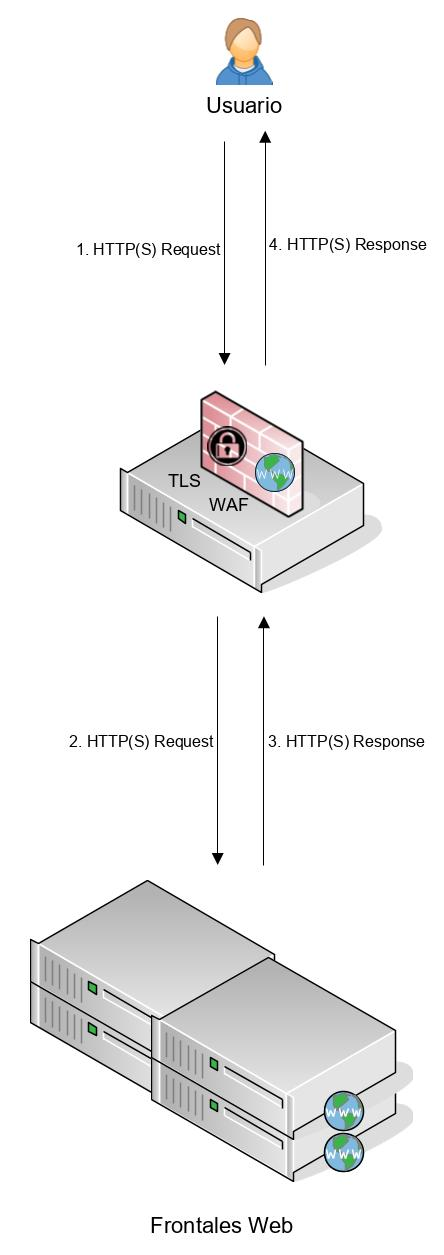
\includegraphics[width=0.3\textwidth]{fig/UseCase1}
        \end{center}
    \end{itemize}
\clearpage
  \item Caso de uso: Petición identificada como no legítima de recurso web.
    \begin{itemize}
      \item Actores: \Gls{Atacante}, plataforma WAF+TLS.
      \item Descripción: Este caso de uso se dará siempre que la plataforma WAF+TLS reciba una petición y la considere un ataque. En este caso se pueden identificar los siguientes pasos:
        \begin{enumerate}
          \item El atacante realiza una petición web a la plataforma WAF+TLS.
          \item La plataforma WAF+TLS recibe la petición, la evalúa y, considerándola como ataque, envía un mensaje de error al atacante.
        \end{enumerate}
        \par A tener en cuenta que la plataforma WAF+TLS ha considerado que el cliente es un atacante y este caso de uso se dará tanto en ataque reales como con falsos positivos (cuando se diagnostica como ataque a una
        petición legítima).
      \item Diagrama:
        \begin{center}
          \label{fig:CasoUso2}
          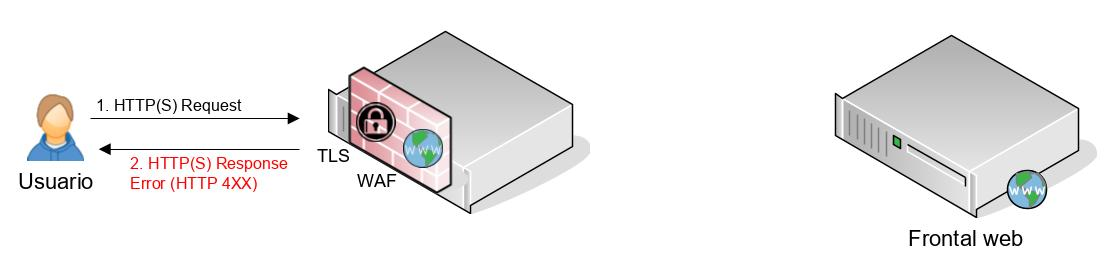
\includegraphics[width=0.3\textwidth]{fig/UseCase2}
        \end{center}
    \end{itemize}
\clearpage
  \item Caso de uso: Petición HTTPS en un entorno con TLS offloading.
    \begin{itemize}
      \item Actores: Cliente, plataforma web, plataforma WAF+TLS.
      \item Descripción: Se trata de una derivada del Caso de primer caso de uso. En este escenario las peticiones HTTPS realizadas por el cliente se envían sin cifrar (o en texto plano) a la plataforma web.
        \par Con ello se consigue reducir la carga que debe soportar la plataforma web y optimizar sus recursos.
        \par Sin embargo, también se aumenta el riesgo a un ataque en caso de que un potencial atacante tuviese acceso a la infraestructura situada entre la solución WAF y la plataforma web. Es por ello que esta solución
        sólo se recomienda en escenarios en los que los elementos situados entre ambos estén protegidos y monitorizados adecuadamente.
      \item Diagrama:
        \begin{center}
          \label{fig:CasoUso3}
          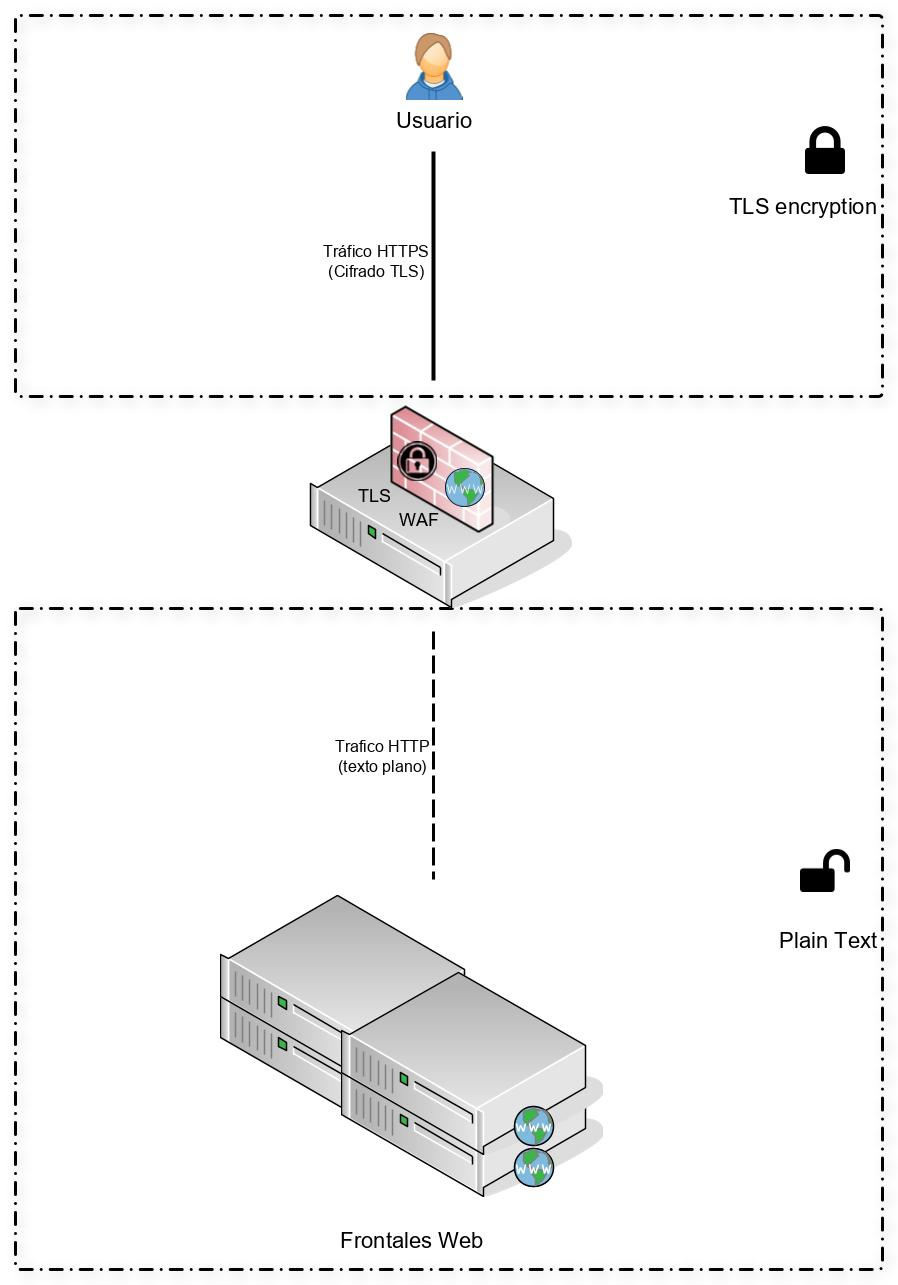
\includegraphics[width=0.7\textwidth]{fig/UseCase3}
        \end{center}
    \end{itemize}
\clearpage
  \item Caso de uso: Petición HTTPS con cifrado punto a punto.
    \begin{itemize}
      \item Actores: Cliente, plataforma web, plataforma WAF+TLS.
      \item Descripción: Se trata de un caso de uso alternativo al anterior. En este escenario se mantienen las comunicaciones cifradas también entre el WAF y la plataforma web, con lo que se consigue el cifrado punto a punto.
        \par Para ello se establecen dos túneles TLS: El primero entre el cliente y la plataforma WAF y un segundo túnel entre el WAF y la plataforma web.
      \item Diagrama:
        \begin{center}
          \label{fig:CasoUso4}
          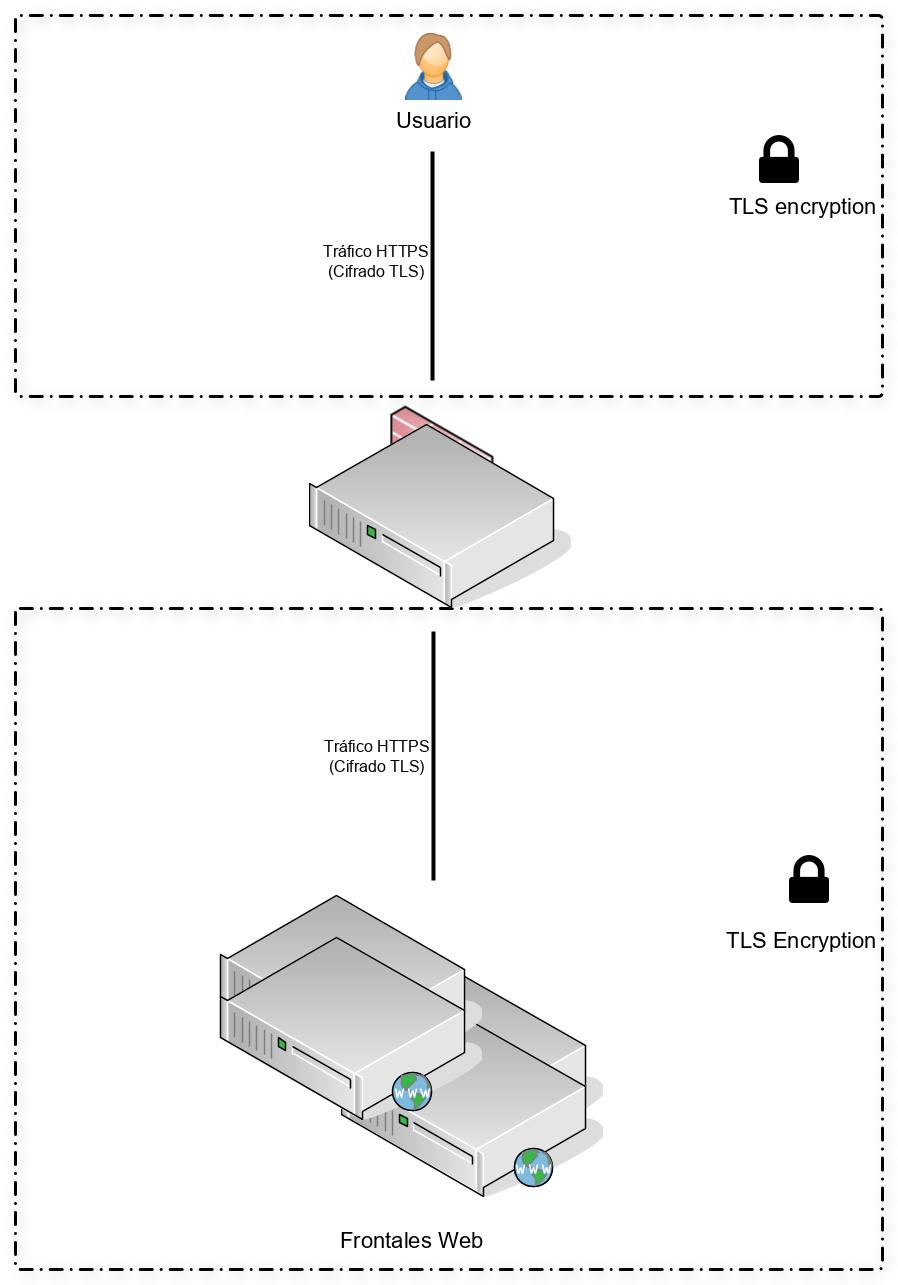
\includegraphics[width=0.7\textwidth]{fig/UseCase4}
        \end{center}
    \end{itemize}
\clearpage
  \item Caso de uso: Petición de validación y firma de certificado TLS a una CA de confianza.
    \begin{itemize}
      \item Actores: \acrlong{ca}, plataforma WAF+TLS.
      \item Descripción: Este caso de uso tiene como objetivo obtener un certificado digitalmente por una \acrshort{ca} que sea de confianza para el cliente. Se puede dividir en dos flujos similares.
        \par El primer flujo se da entre el WAF y la CA siguiendo los siguientes pasos:
        \begin{enumerate}
          \item El WAF - o un administrador del WAF - genera un certificado CSR~\cite[Wikipedia]{wiki:csr} asociado a su clave privada que siga el {\em estándar X.509 v3~\cite[IETF 5280]{rfc5280}}.
          \item Se envía el certificado a la CA solicitando que ésta lo firme.
          \item La CA valida que la petición es legítima y firma el certificado con su clave raíz o, alternativamente, una clave intermedia.
          \item La CA envía el certificado firmado digitalmente el WAF.
          \item Una vez el WAF disponga de dicho certificado, este puede presentar sus servicios web a los clientes y estos podrán validar al WAF durante la negociación TLS si confían en el certificado raíz de la CA o en la
            jerarquía de certificados.
        \end{enumerate}
        \par El segundo flujo es opcional. Se trataría de un flujo similar al descrito para el WAF pero el solicitante de certificado sería la plataforma web en este caso.
        \par Se considera que es opcional debido a que la plataforma web sólo estará expuesta al WAF y se podría crear una relación de confianza sin necesidad de hacer uso de una CA externa.
        \par No obstante, dado que actualmente obtener este tipo de certificados no tiene un coste económico, y que tampoco debería tener un impacto operacional significativo, se recomienda seguir el mismo proceso que para el WAF y
        hacer uso de certificados firmados digitalmente por un CA.
        \par En este proyecto, para la gestión de certificados del WAF se intentará hacer uso del protocolo \acrshort{acme} (\acrlong{acme}) mediante {\em Let’s Encrypt~\cite{letsencrypt}} con el objetivo de automatizar las
        actividades de creación y renovado de certificados.
      \item Diagrama:
        \begin{center}
          \label{fig:CasoUso5}
          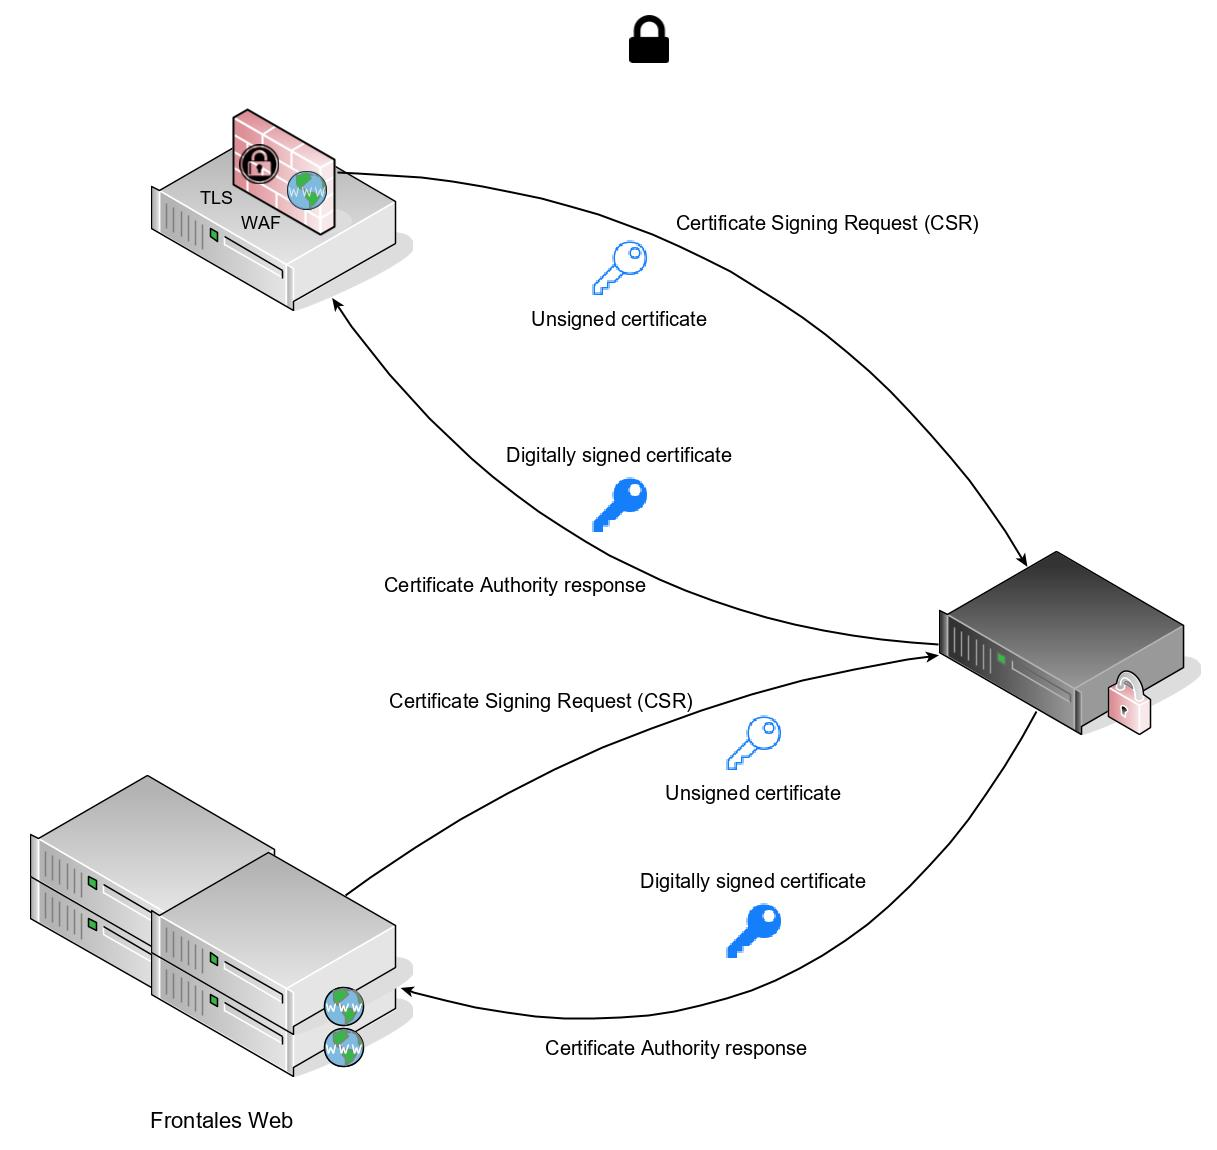
\includegraphics[width=0.7\textwidth]{fig/UseCase5}
        \end{center}
    \end{itemize}
\end{enumerate}




\chapter{Diseño de la solución}
\par Como es habitual en los Proyectos de Fin de Grado, uno de los retos más interesantes que se encuentran consiste en afrontar, abrazar y controlar la
incertidumbre sobre cómo será la solución final; dicha incertidumbre es inherente a todo proyecto de software, pero en un PFG es mayor debido a que la
investigación tiene a su vez un mayor peso y es determinante.
\par En el presente proyecto, a la hora de afrontar inicialmente el diseño de la solución se desconoce qué tecnologías se van a utilizar específicamente y éstas
se deciden tras evaluarlas tanto individualmente como su capacidad de integración entre ellas y con elementos externos.
\par Para ello se sigue un modelo de desarrollo evolutivo similar al modelo de prototipos. Para lo cual se parte de la definición de un diseño a alto nivel en
el que se definen los componentes y sus funciones más representativas. A continuación se empieza a realizar un proceso iterativo en el que se van probando los
componentes y añadiendo nuevos elementos. El resultado de dicha fase es una solución funcional inicial que cumpla los requisitos definidos. Sobre dicho modelo
se realiza una revisión de calidad que permita contar con una solución suficientemente madura y estable.
\par No obstante, dado que se espera que la solución sea algo en constante cambio, se ha elegido una metodología de desarrollo ágil~\cite{wiki:agil}, tal como
se describe más adelante.

\section{Componentes principales}
\par Estos son los componentes que se han identificado para la solución:
\begin{itemize}
  \item El primer componente que se ha identificado es un WAF con licencia de software libre. Este elemento es el componente más importante de la solución y
    marca en gran medida los demás componentes que participen en la capa de aplicación.
    \par Durante la fase de construcción se evalúan qué componentes WAF cumplen los requisitos y se elige un candidato.
  \item El segundo componente de la solución es el software responsable de gestionar las comunicaciones HTTPS. Este software es el encargado de cifrar y
    descifrar el tráfico SSL / TLS.
  \item El tercer componente es el software de virtualización o de contenedores. Uno de los puntos clave de la solución es garantizar la facilidad para
    implementarla de forma poco intrusiva. Para ello se considera que un software de contenedores como Docker~\cite{docker}. Este tipo de soluciones está
    ampliamente asentada en el mercado y existe un movimiento significativo de migración de los entornos tradicionales a entornos de contenedores.
  \item Otro componente estrechamente relacionado con el componente anterior es el software automatización de despliegue y gestión de la solución. Este
    componente es opcional y por lo tanto se tendrá en cuenta que la opción deber ser sustituible en diferentes implementaciones con el fin de garantizar la
    máxima portabilidad de la solución.
  \item Otro componente del que depende la solución es el conector con los elementos de almacenamiento persistente. Este componente es el encargado de
    proporcional un servicio de compartir información entre recursos y garantizar la perdurabilidad de la información necesaria. Se hará foco en reducir el uso
    o impacto de este componente al mínimo y que todo el entorno pueda ser reconstruido con el menor esfuerzo posible con el fin de ofrecer un entorno dinámico
    siguiendo los principios \acrshort{cicd} ya mencionados.
  \item Un componente opcional a considerar es el gestor de certificados HTTPS. Este componente será el responsable de aprovisionar, renovar y revocar certificados que sean confiables para los clientes, por lo que deberá
    comunicarse con una entidad certificadora.
  \item Por último, tenemos dos componentes directamente relacionados con la personalización de la herramienta por el usuario final. Se trata de las reglas de
    auditoría o bloqueo del WAF, así como las reglas de configuración del software de TLS. Estos componentes serán los ficheros o parámetros de configuración de
    los dos primeros componentes que se han identificado.
\end{itemize}

\section{Diseño de alto nivel}
\par Partiendo de los requisitos definidos, se plantea el diseño a alto nivel tal como se muestra en el {~\hyperref[fig:hld]{Diagrama de alto nivel de la solución}} en el que se reflejan los componentes de la solución y
los principales actores.
\begin{figure}[h!]
  \centering
  \label{fig:hld}
  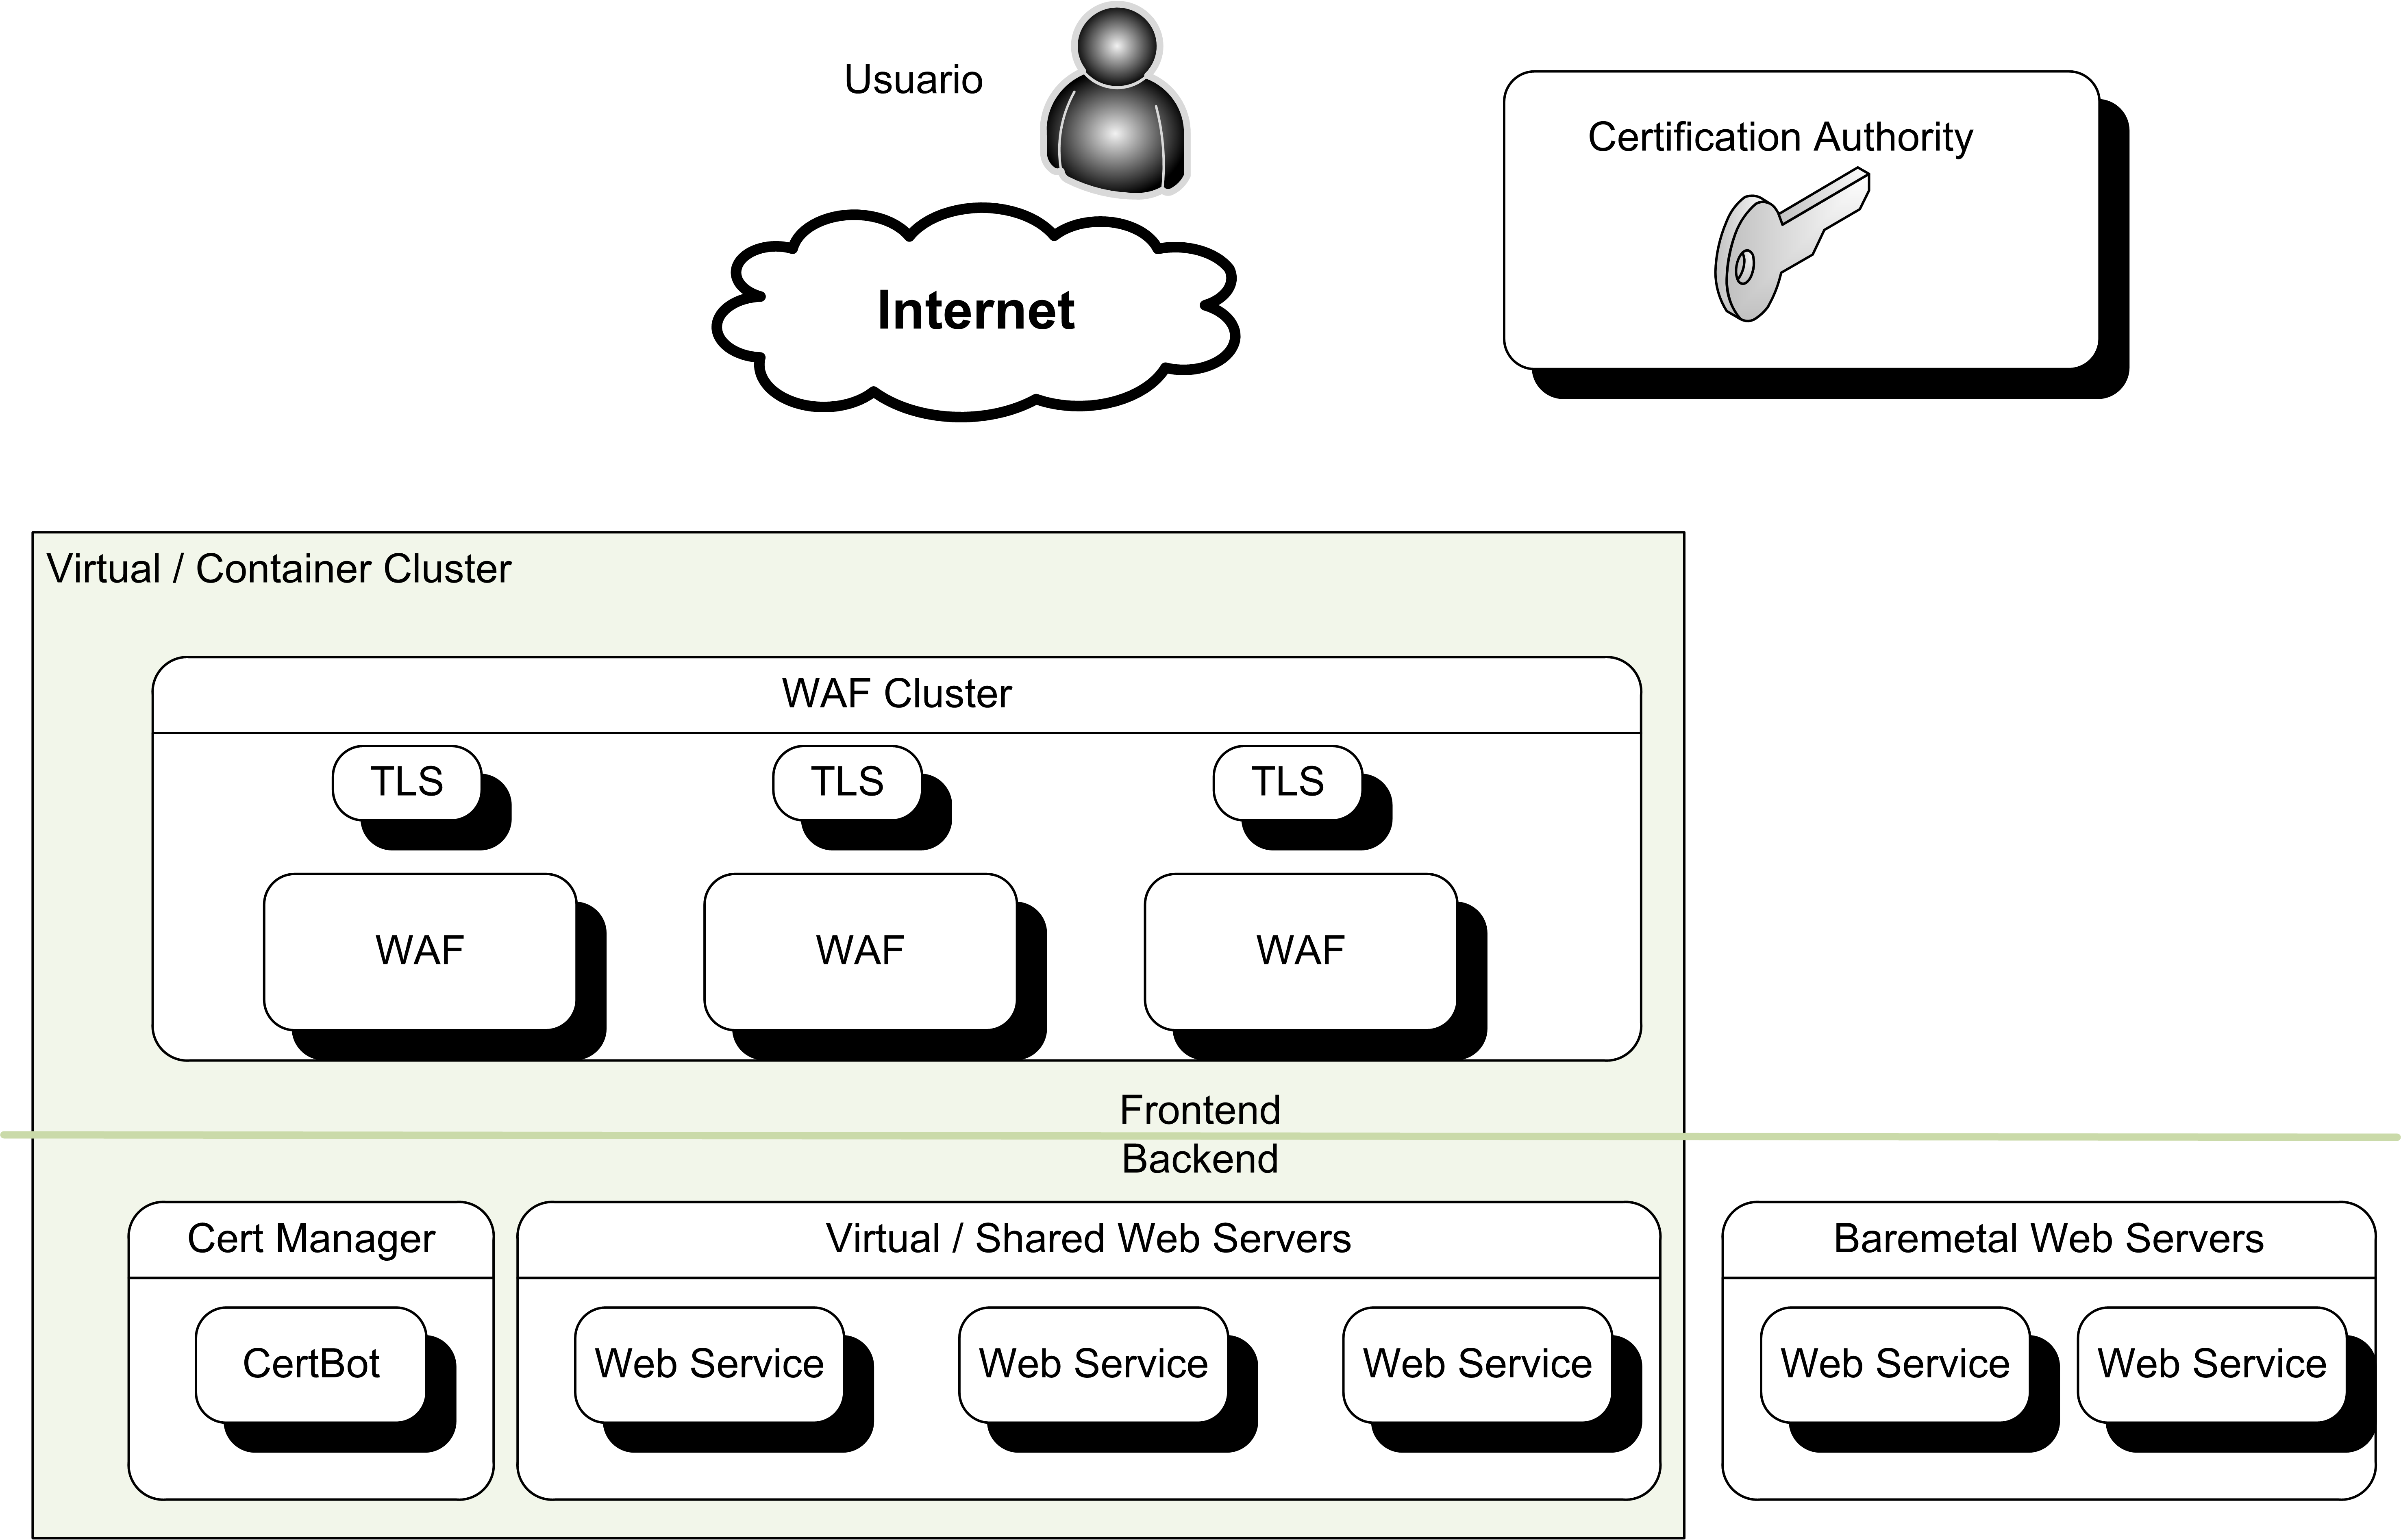
\includegraphics[width=\textwidth]{fig/Diagram_HLD}
  \caption{Diseño de alto nivel}
\end{figure}

\section{Construcción de la solución}
\par Tal como se comentaba anteriormente, debido al alto grado de incertidumbre que se tiene del aspecto final de la solución, junto con la necesidad de poder
realizar cambios sobre el modelo de forma rápida, se ha optado por seguir una metodología de desarrollo ágil~\cite{wiki:agil}.
\par Durante el proceso de desarrollo del proyecto se utilizará como referencia o mantra el \Gls{ManifiestoAgil} y como modelo de liberación de versiones se
siguen los principios de integración continua, entrega continua (en adelante \acrshort{cicd}, de sus siglas en inglés \acrlong{cicd} \cite{cicd}).

\section{Análisis y selección de tecnologías}
\par En esta sección se evalúan las distintas opciones disponibles y se elige una tecnología candidata sobre la que construir la solución.
\subsection{Web Application Firewall}
\par En primer lugar, de acuerdo a los requerimientos establecidos - {~\hyperref[req:softwarelibre]{La plataforma debe ser compatible con el modelo de
licencias de software libre}} - se han descartado las soluciones WAF privativas y aquellas que no estén licenciadas bajo una licencia del tipo GPL.  En
este segundo grupo se encuentran WebKnight - sólo compatible con el software de aplicación web Internet Information Services\cite{iis} sobre plataformas
Microsoft Windows - y Vulture, con licenciamiento BSD y que requiere un sistema operativo FreeBSD.

\par Otras soluciones se han descartado debido a que están discontinuadas desde hace tiempo, como IronBee que no se ha actualizado desde hace más de 3 años
y WebCastellum desde hace 5 años.

\par Otra tecnología candidata que se ha descartado ha sido RAPTOR debido a que no soporta tráfico SSL/TLS ({~\hyperref[req:tls]{La solución debe poder
participar en la negociación TLS}}).

\par NAXSI se ha considerado que no cumple los requisitos básicos que debe tener un WAF actualmente ({~\hyperref[req:commonattacks]{La solución debe
disponer de un conjunto básico de políticas de auditoría o bloqueo que permitan proteger la aplicación web frente a los ataques más comunes}}), pues
sólo implementa dos controles de seguridad - de los referenciados en el documento de buenas prácticas de OWASP\cite[apartado A3.2]{owaspbestpractices});
concretamente, sólo protege ataques de tipo {\em Cross-site scripting} (en adelante \acrshort{xss}\cite{owaspxss}) e inyecciones SQL (en adelante
\acrshort{sqli}\cite{owaspsqli}). Además, se han producido duras críticas acerca de las funcionalidades que ofrece \cite{naxsianalisis}.

\par OpenWAF por su parte es una iniciativa con un planteamiento y unas funcionalidades muy interesantes, pero que lleva más de dos años sin
publicar una nueva versión y además carece de suficiente madurez para considerarse su uso en un entorno de producción (la última versión
publicada es la 0.0.4).

\par Respecto a FreeWAF (también conocido como {\em lua-resty-waf}) está en una situación muy similar a OpenWAF, pues su última versión tiene más de 2
años y se trata de la versión 0.11.1\cite{freewafchangelog}.

\par En el caso de Shadow Daemon, no se cumple el requisito de independencia ({~\hyperref[req:independence]{La solución debe poder ejecutarse en un
sistema operativo o máquina independiente de la plataforma de la aplicación web}}), pues se trata de un conector de aplicación web con una
funcionalidades interesantes, pero por diseño requiere de su integración con el framework de desarrollo y sólo es compatible con PHP, Perl y Python. Por
lo tanto no es posible implementarlo como elemento externo e independiente de la plataforma web.

\par Por último, se ha considerado ModSecurity. Esta tecnología está disponible en dos ramas de desarrollo, la rama 2.x (versión 2.9.3 en el momento en
el que se escribe este documento) y la rama 3.x (versión 3.0.3 actualmente).
\par La rama no cumple los requisitos de independencia ({~\hyperref[req:independence]{La solución debe poder ejecutarse en un sistema operativo o
máquina independiente de la plataforma de la aplicación web}}), debido a que se despliega como un módulo de Apache y no permite que su despliegue sea
agnóstico de la plataforma web; por lo tanto se descarta esta versión de ModSecurity.

\par La rama 3.x por el contrario incorpora entre sus novedades una reescritura completa del código y la posibilidad de enlazarse a distintas
tecnologías de servicios web.

\par Cabe mencionar que las tecnologías que abiertamente no cumplen los requisitos definidos se han descartado, pero aquellas que cumplen con los
requisitos pero que llevan tiempo sin actualizarse o están en una fase temprana de desarrollo se mantienen como opciones alternativas en caso de que la
opción candidata no cumpla con las expectativas.
\subsubsection{Tecnología candidata}
\par Se ha elegido como tecnología candidata ModSecurity en su versión 3.x, pues cumple todos los requisitos y es un referente entre las tecnologías de
WAF de software libre.

\subsubsection{Servicio web}
\par Uno de los componentes sobre los que se debe apoyar el WAF es el servicio web. Este componente se comporta como un interfaz entre el WAF y las peticiones y respuestas del cliente y el servicio web.
\par Se han identificado los siguientes servicios web compatibles con  ModSecurity en su versión 3:
\begin{itemize}
  \item Internet Information Services (IIS)~\cite{iis}.
  \item Apache HTTP Server (Apache)~\cite{apache}.
  \item Nginx~\cite{nginx}.
\end{itemize}
\par IIS se ha descartado debido a que sólo es compatible con plataformas Windows, tal como se comentó en la sección ~\nameref{subsec:estadoarte}.

\par Tanto Apache como Nginx cumplen los requisitos funcionales, pero Nginx tiene mejores capacidades de proxy inverso.

\par Respecto al licenciamiento, Nginx utiliza {\em Licencia BSD simplificada o licencia FreeBSD (de 2 cláusulas)}~\cite{wiki:SimplifiedBSDLicense}, la cual es compatible con GPL.

\subsubsection{Tecnología candidata}
\par Se ha elegido como servicio web Nginx.

\subsection{Software criptográfico}
\par Uno de los puntos clave para proporcionar un canal cifrado y seguro alineado con las mencionadas mejores prácticas de TLS ~\cite{TLSBestPractices} o de PCI DSS~\cite{pcidssrequirements} es el uso de TLS en su versión 1.3 y HTTP/2.
\par Se han descartado por lo tanto las soluciones que no cumplen estos requisitos, como por ejemplo LibreSSL~\cite{libressl}.
\par Una vez realizado este primer filtro, se han seleccionado las siguientes opciones:
\begin{itemize}
  \item GnuTLS~\cite{gnutls}.
  \item OpenSSL~\cite{openssl}.
  \item Network Security Services (NSS~\cite{nss}).
\end{itemize}

\par A la hora de valorar estas opciones se ha identificado que a nivel de licenciamiento, sólo GnuTLS utiliza una licencia de tipo GPL.
\par Sin embargo, uno de los componentes previamente seleccionados - Nginx - sólo es compatible con OpenSSL~\cite{opensslnginx}.
\par OpenSSL por su parte tiene una licencia doble, licencia ~\cite[Apache License 1.0]{apachelicense10} y \cite[licencia SSLeay]{ssleaylicense}, esta última heredada del proyecto original en el que se basa OpenSSL.

\par Para resolver este problema se han identificado diferentes opciones:
\begin{enumerate}
  \item Cambiar Nginx por una alternativa que soporte GnuTLS.
  \item Desplegar los componentes de cifrado y de WAF en sistemas independientes.
  \item Revisar la compatibilidad de licencias.
\end{enumerate}

\par Para evaluar la viabilidad de la primera opción se han identificado qué servicios son compatibles con GnuTLS. Según la Wikipedia~\cite{wiki:gnutls} este proyecto es usado principalmente en clientes TLS y sólo es compatible con el servicio
web Apache, el cual a su vez tiene el mismo tipo de licencia que OpenSSL (Apache License). Por lo que tiene la misma incompatibilidad de licencias ya mencionada.

\par Debido a la falta de compatibilidad de GnuTLS con otros servicios web, la segunda opción mantiene la dependencia de Apache y su licencia, por lo que  se debe descartar igualmente esta opción.

\par Para evaluar la tercera opción, dado que la librería OpenSSL es una de las más utilizadas, se ha investigado cual es el acercamiento que otros proyectos de software libre.
\par El acercamiento de algunos proyectos es utilizar una licencia tipo GPL modificada en la que se añade una excepción para esta librería~\cite{opensslexception}. Esta solución la han seguido proyectos como {\em GNU Wget} y {\em climm}. Para
ello se deben adjuntar archivos binarios dentro del proyecto y modificar la licencia GPL ofrecida por la GNU; si bien es una opción viable, no es la opción deseable.
\par Investigando cual es el acercamiento de otros proyectos para mantener su licencia GPL y utilizar OpenSSL, se ha identificado que OpenSSL ha iniciado un proceso de cambio de licencia para atajar este problema. Para ello han decidido
cambiar su licencia por una compatible con GPL (~\cite[Anuncio del cambio de licencia]{opensslannouncement}). El cambio de licencia se ha aplicado recientemente (\cite[{\em Pull request} del cambio]{opensslpullrequest}) y ya es efectivo en las
versiones proporcionadas por la versión {\em Buster} de Debian GNU/Linux.
\par Con este cambio se elimina la incompatibilidad de licencias que se había identificado.

\subsubsection{Tecnología candidata}
\par Se ha elegido como tecnología candidata OpenSSL, pues cumple todos los requisitos y es una de las librerías más extendidas y probadas.

\subsection{Software de virtualización}
\par A la hora de elegir software de virtualización, todas las soluciones que se conocen cumplen con los requisitos y objetivos del proyecto, por lo que se ha optado por Docker debido a que es una solución ampliamente utilizada y en constante
expansión.

\subsubsection{Tecnología candidata}
\par La solución que se ha elegido es \cite{docker}.

\par Dentro de cada instancia del contenedor Docker se desplegará Nginx y ModSecurity y OpenSSL:
\begin{figure}[!h]
  \centering
  \label{fig:Diagram_WAF_TLS}
  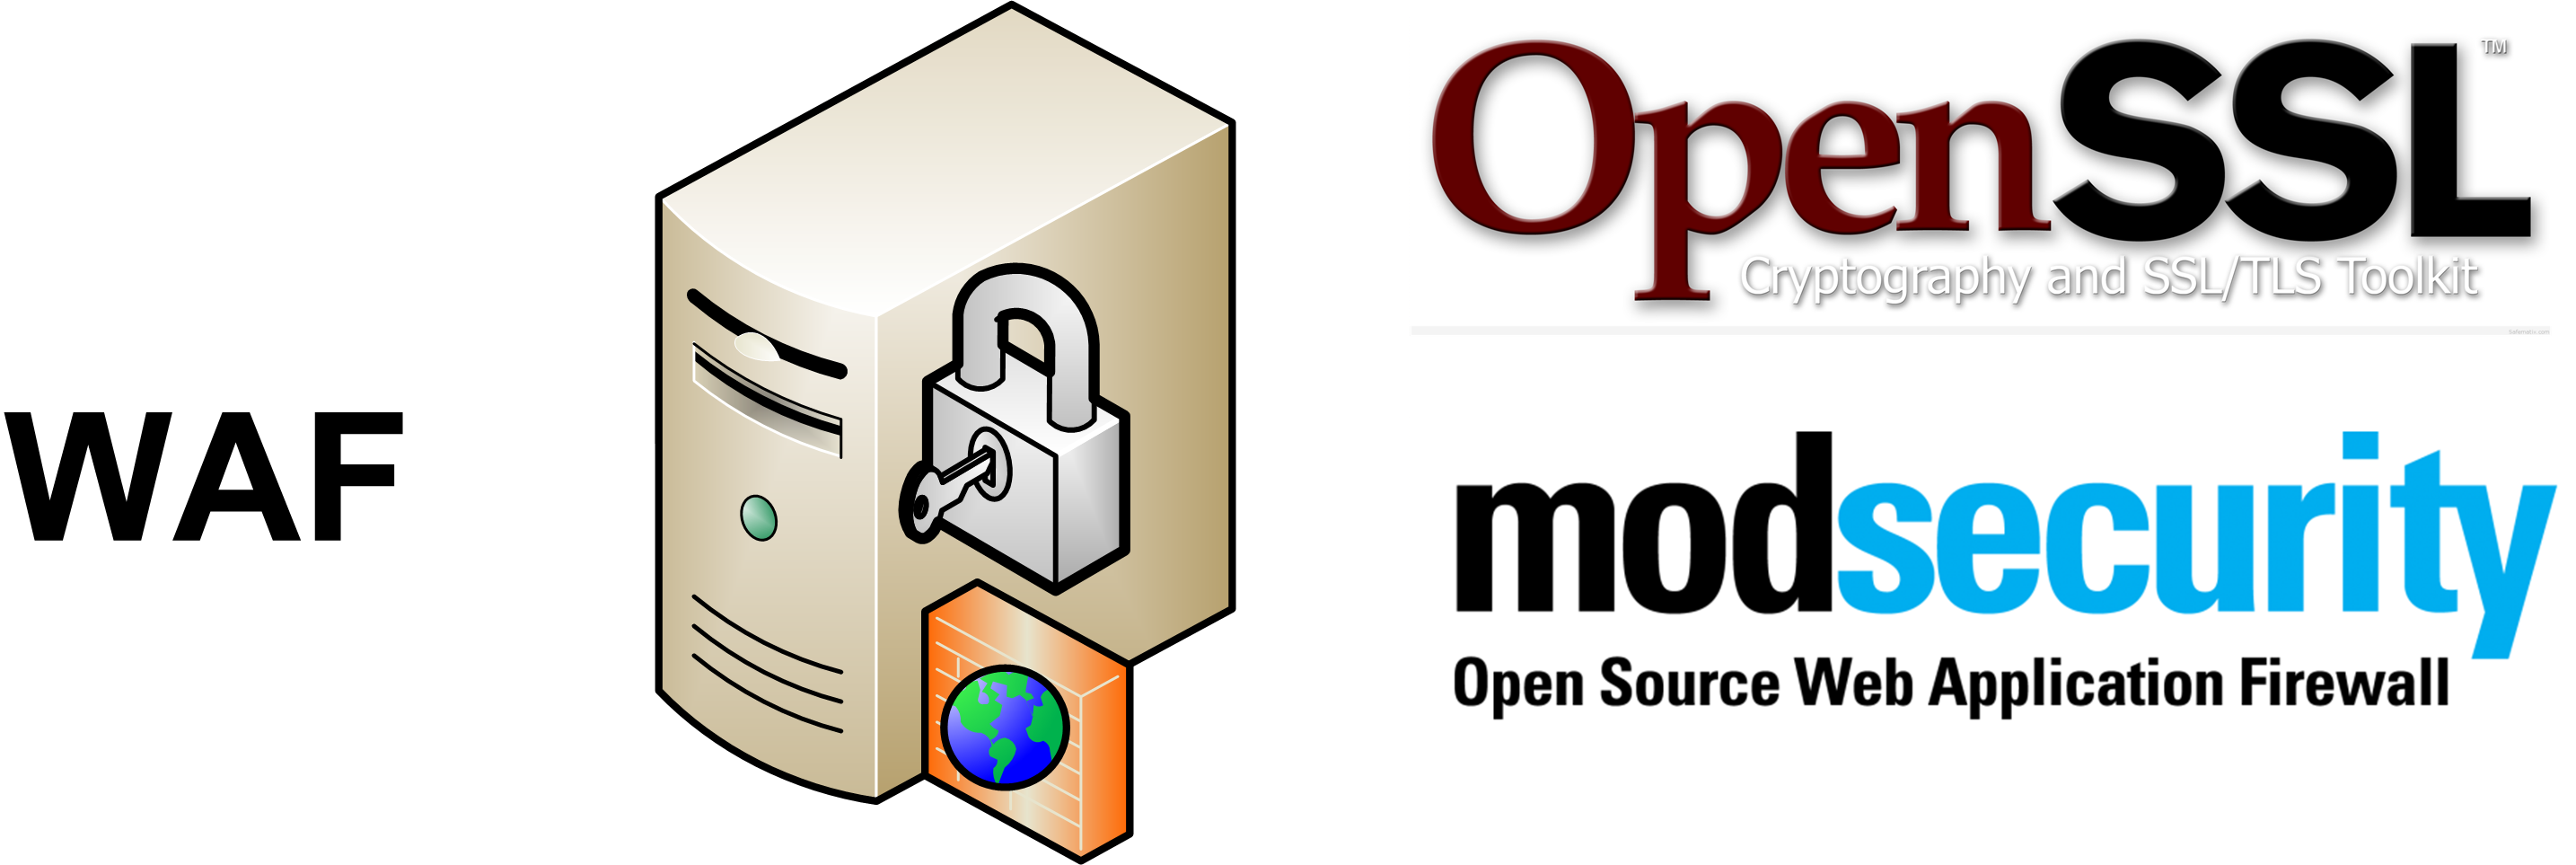
\includegraphics[width=0.7\textwidth]{fig/Diagram_WAF_TLS}
  \caption{Componentes desplegados en cada instancia WAF}
\end{figure}

\subsection{Software de automatización u orquestación}
\par Esta tecnología será la responsable de garantizar el cumplimiento de los siguientes requisitos:
{~\hyperref[req:facilidad]{La plataforma debe ser fácilmente integrable en la plataforma web del cliente.}}
{~\hyperref[req:escalado]{Escalabilidad. La plataforma debe permitir la ampliación o reducción de recursos de forma dinámica.}}

\par Para poder ofrecer estas funcionalidades, se han evaluado las siguientes tecnologías:
\begin{itemize}
  \item Kubernetes (K8s)~\cite{kubernetes}.
  \item Apache Mesos~\cite{mesos}.
  \item Docker Swarm~\cite{swarm}.
\end{itemize}

\par Todas las tecnologías cumplen las necesidades funcionales definidas y todas ellas tiene un licenciamiento compatible con las licencias de tipo GPL.

\par Para poder ofrecer que la solución sea fácilmente integrable, se ha evaluado el uso de estas soluciones y se ha comprobado como Kubernetes es la solución más ampliamente extendida (ver los gráficos
{~\hyperref[fig:KubernetesSwarm]{Kubernetes y Docker Swarm}} y {~\hyperref[fig:KubernetesMesos]{Kubernetes y Apache Mesos}}).

\begin{figure}[!htb]
  \centering
  \begin{subfigure}[t]{.45\textwidth}
    \centering
    \label{fig:KubernetesSwarm}
    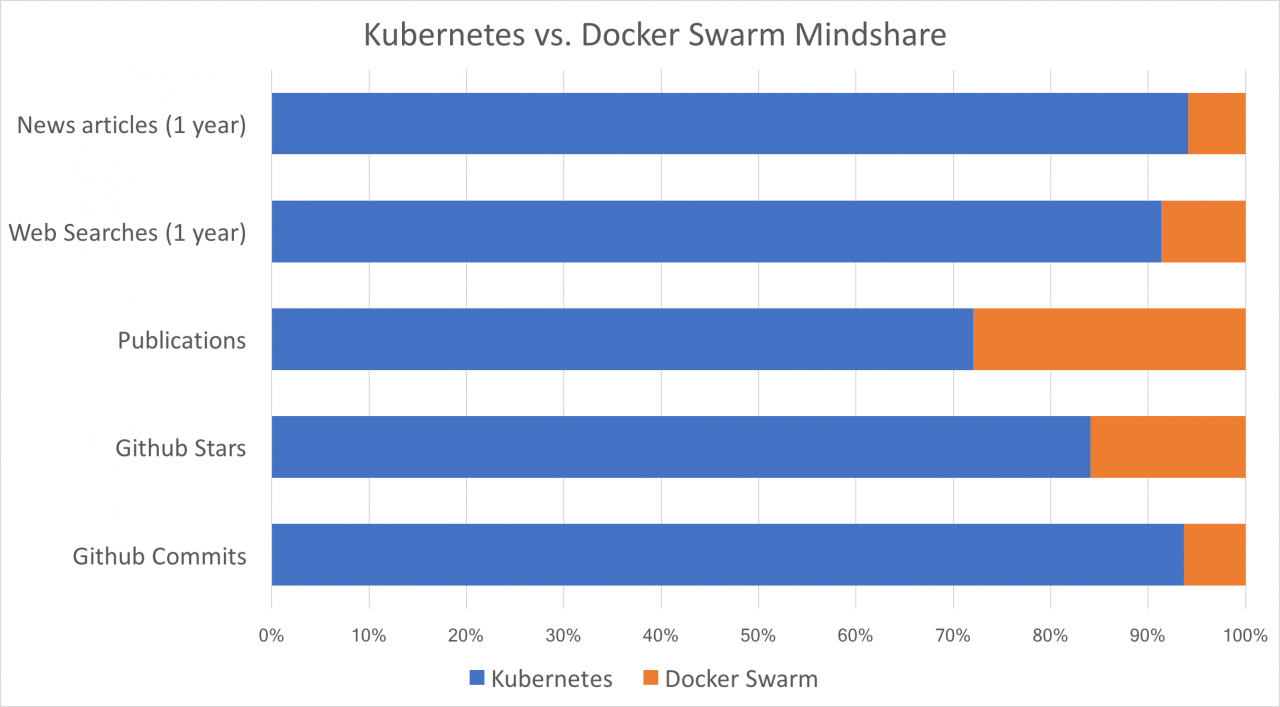
\includegraphics[width=\textwidth]{fig/KubernetesSwarm}
    \caption{Uso y popularidad de software de Kubernetes y Docker Swarm(fuente Platform9~\cite{KubernetesSwarm})}
  \end{subfigure}
  \hfill
  \begin{subfigure}[t]{.45\textwidth}
    \centering
    \label{fig:KubernetesMesos}
    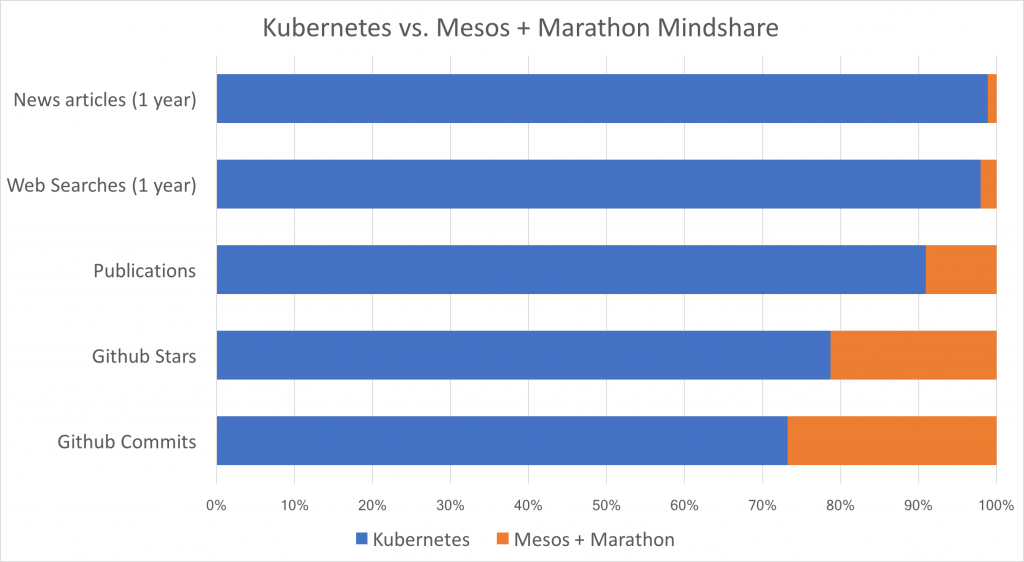
\includegraphics[width=\textwidth]{fig/KubernetesMesos}
    \caption{Uso y popularidad de software de Kubernetes y Apache Mesos(fuente Platform9~\cite{KubernetesMesos})}
  \end{subfigure}
\end{figure}

\par Si además comparamos la evolución que estas tecnologías han tenido históricamente, la diferencia es aun mayor como se puede comprobar en el gráfico de {~\hyperref[fig:orquestatorspopularity]{Popularidad de software de orquestación}}. 
\begin{figure}[!htb]
  \centering
  \label{fig:orquestatorspopularity}
  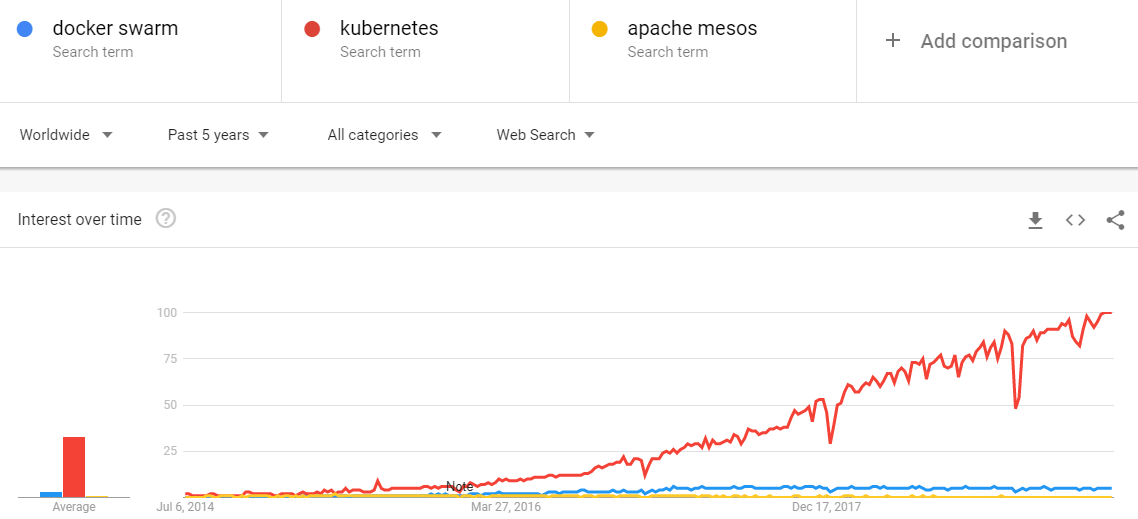
\includegraphics[width=0.7\textwidth]{fig/KubernetesSwarmMesos}
  \caption{Histórico de popularidad de software de orquestación (fuente Google~\cite{KubernetesSwarmMesos})}
\end{figure}

\par Cabe mencionar que existen soluciones Kubernetes adaptadas a los entornos de los principales proveedores del Cloud, como son {\em Azure Kubernetes Service (AKS)~\cite{aks}} o
{\em Amazon Elastic Kubernetes Service (Amazon EKS)~\cite{eks}}. Estas soluciones cuentan con la ventaja de que facilitan su despliegue y mantenimiento mediante
el uso de herramientas propias, pero cuentan con una fuerte desventaja: Aumentan la cautividad de la solución con un único proveedor.
\par Sin embargo, la migración de una solución agnóstica del proveedor del Cloud a un proveedor específico es sencilla.
\par Por lo tanto se ha optado por no utilizar ninguna solución específica del Cloud y utilizar la tecnología Kubernetes sin funcionalidades añadidas como son
los {\em Ingress Controllers~\cite{ingresscontrollers}} o API de proveedores del Cloud. Esto permitirá que la solución sea fácilmente desplegable en el mayor
número de entornos posible.

\subsubsection{Tecnología candidata}
\par Se ha elegido Kubernetes~\cite{kubernetes} como tecnología candidata para implementar la automatización de la plataforma.

\par Kubernetes será responsable de desplegar las instancias WAF que sean necesarias, garantizar su disponibilidad y volver a desplegarlas si hubiese algún problema con alguna de ellas.

\subsection{Servicio de almacenamiento}
\par El objetivo de este componente es garantizar un servicio de intercambio de información entre los distintos componentes de la misma y, en caso de que sea
necesario, el almacenamiento persistente de la información. Pero, tal como se ha comentado anteriormente, se intentará minimizar su uso. De ser posible se
utilizará alguna solución ya presente en la infraestructura.
\par Entre las soluciones a evaluar existen dos aproximaciones posibles: Servicios tradiciones como Samba ~\cite{samba} o  NFS (estándar RFC7530~\cite{nfs}) o
servicios del Cloud como Amazon S3\cite{s3} o Google Storage\cite{GoogleStorage}.

\par Tal como se ha identificado a la hora de identificar la tecnología de automatización, las soluciones proporcionadas por los fabricantes del Cloud limitan
las posibles plataformas que adopten la solución, por lo que se prefiere utilizar servicios de almacenamiento e intercambio de archivos independientes del
proveedor.
\par Tanto Samba como NFS cubren los requisitos, por lo que cualquiera de estas tecnologías son válidas. Sin embargo, dentro de los entornos de contenedores el
protocolo NFS está más extendido.

\subsubsection{Tecnología candidata}
\par Se utilizará por tanto un servicio de almacenamiento basado en ~\cite{nfs}, preferiblemente un recurso externo a la solución propuesta.

\subsection{Políticas o reglas de auditoría}

\subsubsection{Tecnología candidata}



\section{Arquitectura}
\par Tal como se ha comentado anteriormente, se procede a construir la solución de forma iterativa.
\par Debido a las funcionalidades añadidas por las últimas versiones del software, se utilizarán las últimas versiones estables de todo el software, para lo cual se descargará el código fuente y compilará según se
requiera.
\par Esto permite a su vez minimizar las dependencias entre la solución y el sistema operativo, lo que facilitará que ésta se adapte a otros sistemas si así se requiere.
\par No obstante, se utilizará como base un sistema operativo Debian GNU/Linux.

\subsection{Web Application Firewall}
\par El primer componente que se debe construir es el \acrshort{waf}. Para ello, se han definido las siguientes capas de seguridad:
\begin{enumerate}
  \item {\bf ModSecurity}. Es la primera capa de seguridad y la funcionalidad que propiamente se considera como WAF.
    \par Se utilizarán las reglas de WAF definidas por OWASP~\cite{owaspcrs}.
  \item {\bf Seguridad de la Cookie}. Se aplicarán una serie de atributos con el fin de evitar el robo o uso indebido de cookies.
  \item {\bf Cabeceras HTTP de seguridad}. Se aplicarán una serie de cabeceras HTTP que protegen contra diversos ataques.
  \item {\bf Cabecera \acrlong{hsts} (\acrshort{hsts})}. Esta cabecera HTTP evita que se realicen peticiones mediante canales no cifrados.
  \item {\bf HTTP/2}. La versión 2 de HTTP aporta una serie de mejoras respecto a las versiones anteriores en materia de seguridad y de rendimiento.
\end{enumerate}

\clearpage
\par El WAF constará pues de los componentes identificados en el {~\hyperref[fig:Diagrama_WAF_Componentes]{Diagrama del \acrshort{waf}}}
\begin{figure}[!ht]
  \centering
  \label{fig:Diagrama_WAF_Componentes}
  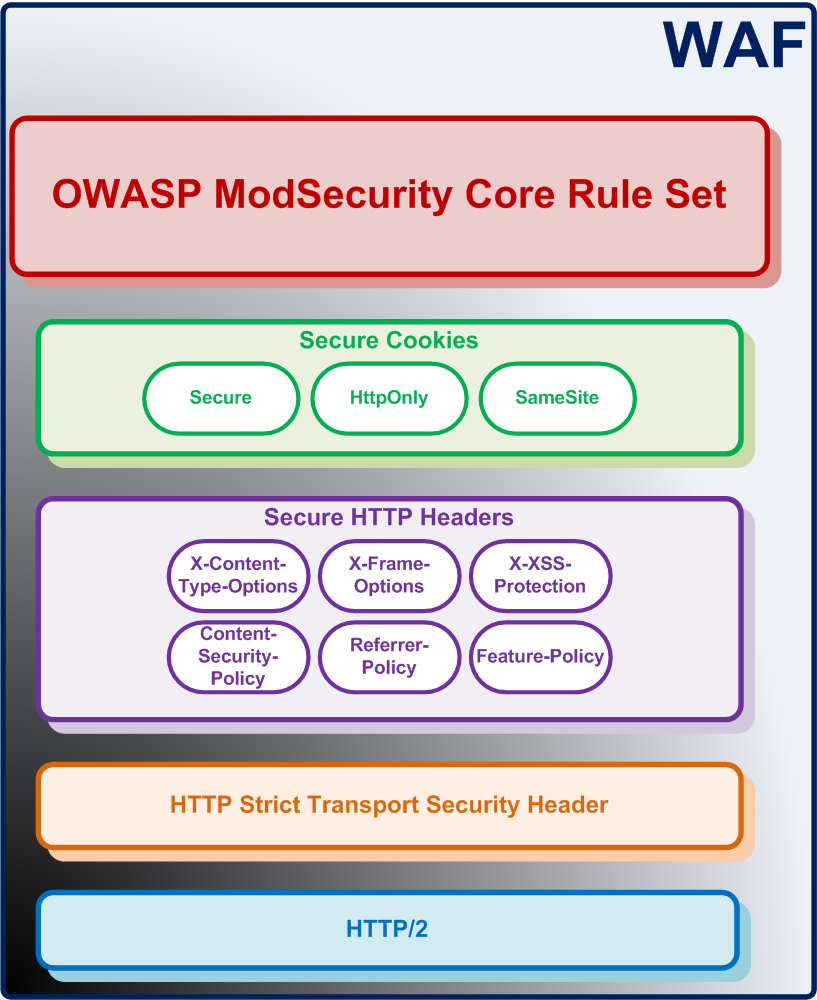
\includegraphics[width=0.7\textwidth]{fig/Diagrama_WAF_Componentes}
  \caption{Diseño de alto nivel}
\end{figure}

\subsubsection{Construcción de ModSecurity}
\par Se procede a construir el componente base sobre el que se basarán los demás componentes, esto es un WAF sobre Nginx.
\par En primer lugar se debe instalar el conector de ModSecurity.
  \lstinputlisting[language=bash,firstline=13,lastline=14]{\codePath/Docker/ccwaf/files/build/build_nginx.sh}

\par A continuación se procede a descargar e instalar la última versión disponible de Nginx. \\
\begin{minipage}{\linewidth}
  \lstinputlisting[language=bash,linerange={21-25,27-33,35-40}]{\codePath/Docker/ccwaf/files/build/build_nginx.sh}
\end{minipage}

\par Se descarga e instala ModSecurity. \\
\begin{minipage}{\linewidth}
\begin{lstlisting}[language=bash]
cd /opt/ \
git clone https://github.com/SpiderLabs/ModSecurity \
cd ModSecurity/ \
git checkout -B v3/master origin/v3/master \
sh build.sh \
git submodule init \
git submodule update \
./configure \
make \
make install \
\end{lstlisting}
\end{minipage}

\par Por último, se configura ModSecurity con una regla de bloqueo que permita realizar pruebas.\\
\begin{minipage}{\linewidth}
  \lstinputlisting[language=bash,firstline=3,lastline=33]{\codePath/Docker/ccwaf/files/build/build_modsecurity.sh}
\end{minipage}
\par El WAF envía una respuesta HTTP 403 cuando se aplica dicha regla a la petición tal como se ve en la captura ({~\hyperref[fig:WAF_test]{Respuesta de WAF a una petición no legítima}}).

\begin{figure}[!ht]
  \centering
  \label{fig:WAF_test}
  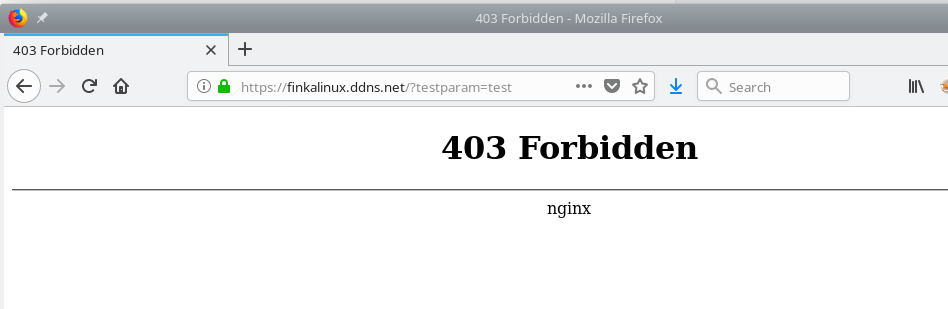
\includegraphics[width=0.7\textwidth]{fig/WAF_testparam}
  \caption{Respuesta de WAF a una petición no legítima. }
\end{figure}

\subsubsection{Soporte HTTP/2}
\par El siguiente componente que se debe añadir es el soporte en Nginx mediante el parámetro \\ \lstinline{--with-http_v2_module}.

\par Por lo que se debe compilar Nginx con los siguientes parámetros:\\
\begin{minipage}{\linewidth}
  \lstinputlisting[language=bash,linerange={24-25,27-40}]{\codePath/Docker/ccwaf/files/build/build_nginx.sh}
\end{minipage}

\par A continuación se debe  habilitar el protocolo en el fichero de configuración de nginx ({\em nginx.conf}).
\par Para ello, se modifica el parámetro {\em listen} del bloque {\em server} destinado a HTTPS:
\begin{lstlisting}[language=bash]
listen        443 ssl http2 default_server;
listen        [::]:443 ssl http2 default_server;
\end{lstlisting}

\par La segunda línea se añade con el fin de que la solución tenga soporte para IPv6.

\subsubsection{Cabecera HTTP Strict Transport Security}
\par La cabecera \acrlong{hsts}~\cite{wiki:hsts}(\acrshort{hsts} en adelante) permite implantar una política de seguridad que obliga al cliente a comunicarse mediante canales cifrados SSL/TLS.
\par Esto permite proteger el tráfico frente a ataques que puedan interceptar las comunicaciones como por ejemplo un {\em ataque de intermediario} o \gls{MitM} (en adelante \acrshort{mitm}).
\par Para habilitar esta política, se añade la siguiente cabecera a la configuración:
\begin{lstlisting}[language=bash]
add_header Strict-Transport-Security "max-age=31536000; includeSubDomains" always;
\end{lstlisting}
\par Los parámetros especificados son los siguientes:
\begin{itemize}
\item  \lstinline{max-age=31536000}. Indica la duración de la política en el cliente web. En este caso un año.
\item  \lstinline{includeSubDomains}. Indica que dicha política se debe aplicar a todos los subdominios.
\item  \lstinline{always}. Indica que la política se debe añadir a cualquier tipo de respuesta HTTP.
\end{itemize}

\subsubsection{Cabecera de seguridad {\em X-Content-Type-Options}}
\par La siguiente cabecera que se añade es {\em X-Content-Type-Options}~\cite{X-Content-Type-Options}. Esta cabecera previene que un cliente pueda realizar {\em MIME type sniffing}~\cite{mimesnif}. Esta funcionalidad representa un riesgo de seguridad debido a que permite potencialmente transformar un tipo MIME no ejecutable en ejecutable.
\par Para habilitar esta política, se añade la siguiente cabecera a la configuración:
\begin{lstlisting}[language=bash]
add_header X-Content-Type-Options "nosniff" always;
\end{lstlisting}
\par El parámetro \lstinline{nosniff} previene que el cliente aplique un tipo MIME diferente al indicado por el servidor web.
\par El parámetro \lstinline{always} tiene un comportamiento similar a lo descrito en otras cabeceras.


\subsubsection{Cabecera de seguridad {\em X-Frame-Options}}
\par Otra cabecera de seguridad a habilitar es {\em X-Frame-Options}~\cite{X-Frame-Options}. Esta cabecera previene que la petición se enmarque dentro de un frame/iframe de un dominio que no haya sido autorizado, una
técnica habitual en los ataques del tipo \gls{Clickjacking}.
\par Para habilitar esta política, se añade la siguiente cabecera a la configuración:
\begin{lstlisting}[language=bash]
add_header X-Frame-Options SAMEORIGIN always;
\end{lstlisting}
\par El parámetro \lstinline{SAMEORIGIN} indica que las peticiones sólo podrán realizarse en frames/iframes pertenecientes al mismo dominio.


\subsubsection{Cabecera de seguridad {\em X-XSS-Protection}}
\par La siguiente cabecera que se habilita es {\em X-XSS-Protection}~\cite{X-XSS-Protection}. Esta cabecera indica al navegador web que habilite y aplique el filtro contra vulnerabilidades del tipo \gls{XSS}.
\par Para habilitar esta política, se añade la siguiente cabecera a la configuración:
\begin{lstlisting}[language=bash]
add_header X-XSS-Protection "1; mode=block" always;
\end{lstlisting}
\par El parámetro \lstinline{1; mode=block} indica que el filtro contra vulnerabilidades XSS debe estar activado obligatoriamente.


\subsubsection{Cabecera de seguridad {\em Referrer-Policy}}
\par La cabecera {\em Referrer-Policy}~\cite{ReferrerPolicy} tiene como función limitar qué información se envía en la cabecera {\em Referrer}.
\par Esta cabecera se envía cuando el usuario hace click en un enlace y, por defecto, se envía la URL completa de la página actual a la nueva página. Esto implica que, si existe algún tipo de información en la URL actual, la
página web destino tendrá acceso a ella.
\par Este comportamiento puede aprovecharse para realizar ataques de falsificación de petición en sitios cruzados (en adelante \acrshort{xsrf}, del inglés \gls{xsrf}) o \gls{Phishing} entre otros.
\par Para habilitar esta política, se añade la siguiente cabecera a la configuración:
\begin{lstlisting}[language=bash]
add_header Referrer-Policy "strict-origin-when-cross-origin";
\end{lstlisting}
\par El parámetro \lstinline{strict-origin-when-cross-origin} indica lo siguiente:
\begin{itemize}
  \item Si la dirección destino es más insegura que la dirección actual (HTTPS $\rightarrow$ HTTP), no se envía ningún dato en la cabecera {\em Referrer}.
  \item Si la dirección destino pertenece al mismo dominio, se envía la URL completa.
  \item Si la dirección destino pertenece a un dominio diferente, se enviará el dominio de la dirección actual y se eliminará cualquier parámetro o ruta de la URL.
\end{itemize}

\subsubsection{Cabecera {\em Feature-Policy}}
\par La cabecera {\em Feature-Policy}~\cite{FeaturePolicy} define las funcionalidades permitidas. Se trata de una política bastante reciente cuyo borrador ha sido publicado por el \acrshort{w3c} (\acrlong{w3c}) en abril de 2019~\cite{FeaturePolicyDraft}.
\par Actualmente se han publicado las siguientes directivas:
\begin{multicols}{2}
\begin{itemize}
	\item ambient-light-sensor
	\item autoplay
	\item accelerometer
	\item camera
	\item display-capture
	\item document-domain
	\item encrypted-media
	\item execution-while-not-rendered
	\item execution-while-out-of-viewport
	\item fullscreen
	\item geolocation
	\item loading-frame-default-eager
	\item loading-image-default-eager
	\item gyroscope
	\item magnetometer
	\item microphone
	\item midi
	\item payment
	\item picture-in-picture
	\item speaker
	\item sync-xhr
	\item usb
	\item wake-lock
	\item vr / xr
\end{itemize}
\end{multicols}

\par Se han definido las siguientes políticas con el fin de garantizar compatibilidad sin sacrificar la seguridad. \\
\begin{minipage}{\linewidth}
  \lstinputlisting[language=bash,firstline=103,lastline=116]{\codePath/Docker/ccwaf/files/nginx_conf/snippets/security_headers.conf}
\end{minipage}

\par Los valores elegidos son:
\begin{itemize}
  \item \lstinline{'self'}. Indica que la funcionalidad está permitida en las peticiones al dominio y en peticiones dentro de los iframes que pertenezcan al mismo dominio.
  \item \lstinline{'none'}. Indica que la funcionalidad no está permitida.
\end{itemize}

\par Se espera ir ajustando los parámetros a medida que se implementen estas políticas en distintos entornos y evolucionen las directivas.


\subsubsection{Cabecera de Políticas de Seguridad de Contenido}
\par La cabecera de Políticas de Seguridad de Contenido~\cite{csp} (en adelante \acrshort{csp}, del inglés \acrlong{csp}) define una serie de directivas de seguridad que permiten proteger la plataforma
de ataques \gls{XSS} o \gls{SQLI}.
\par Estas políticas son muy versátiles pero también pueden provocar que el contenido no se entregue adecuadamente.
\par Para prevenirlo, se ha identificado el contenido multimedia y las redes sociales más comunes:
\begin{multicols}{2}
\begin{itemize}
  \item 500px.com
  \item 500px.org
  \item cloudflare.com
  \item facebook.com
  \item facebook.net
  \item flickr.com
  \item google-analytics.com
  \item googleapis.com
  \item google.com
  \item imgur.com
  \item jquery.com
  \item reddit.com
  \item staticflickr.com
  \item youtube.com
\end{itemize}
\end{multicols}

\par Utilizando estos servicios como referencia, se han codificado las siguientes listas: \\
\begin{minipage}{\linewidth}
  \lstinputlisting[language=bash,linerange={40-70}]{\codePath/Docker/ccwaf/files/nginx_conf/snippets/security_headers.conf}
\end{minipage}

\par Por último, se ha configurado y habilitado la cabecera \acrshort{csp} como se muestra a continuación: \\
\begin{minipage}{\linewidth}
  \lstinputlisting[language=bash,linerange={77-82,85-88}]{\codePath/Docker/ccwaf/files/nginx_conf/snippets/security_headers.conf}
\end{minipage}

\subsubsection{Control de seguridad de {\em Cookies}}
\par Otro elemento que se deben proteger son las cookies de la plataforma web (\gls{Cookie}), para ello el WAF modificará las cookies de la plataforma web añadiendo los siguientes atributos si no estuviesen previamente:
\begin{itemize}
  \item Secure. Previene que la cookie sea enviada mediante canales no cifrados.
  \item HttpOnly. Previene que la cookie sea accesible por un medio que no sea HTTP/HTTPS. Por lo tanto la cookie no puede ser accesible por un script en el navegador, lo que proporciona protección contra ataques de
    \acrshort{xss}.
  \item SameSite. Previene que la cookie se envíe a un dominio diferente, por lo que ayuda a proteger la plataforma frente a ataques \gls{XSRF}.
    \par Debido a que es una práctica habitual el uso de la misma cookie en distintos dominios se ha optado por aplicar este filtro en una modalidad más permisiva: \lstinline{SameSite=Lax}. Esta opción evita que se envíe
    la cookie en peticiones POST entre otras.
\end{itemize}

\par Nginx por defecto soporta esta funcionalidad para la pagina raíz ("{\em /}"), pero esta protección no se aplica a las demás páginas.
\par Para solucionarlo se hace uso de un módulo externo, \lstinline{nginx_cookie_flag_module}~\cite{nginx_cookie}, con este módulo se pueden habilitar los atributos identificados a todas las cookies con independencia de la URL.
\par En primer lugar se debe descargar el módulo.
  \lstinputlisting[language=bash,firstline=17,lastline=18]{\codePath/Docker/ccwaf/files/build/build_nginx.sh}

\par A continuación se debe modificar la compilación de Nginx añadiendo el siguiente parámetro \\ \lstinline{--add-module=../nginx_cookie_flag_module}.

\par Y se compila Nginx con los siguientes parámetros:\\
\begin{minipage}{\linewidth}
  \lstinputlisting[language=bash,linerange={24-38}]{\codePath/Docker/ccwaf/files/build/build_nginx.sh}
\end{minipage}

\subsection{Software criptográfico}
\par Se procede a configurar las comunicaciones HTTPS.
\par Para ello, lo primero será crear un certificado auto-firmado de pruebas con su correspondiente clave privada. \\
\begin{minipage}{\linewidth}
  \lstinputlisting[language=bash,linerange={3-10,65-67}]{\codePath/Docker/ccwaf/files/build/build_nginx.sh}
\end{minipage}

\par A continuación se debe configurar Nginx para que ofrezca este certificado a los clientes.\\
\begin{minipage}{\linewidth}
  \lstinputlisting[language=bash,linerange={29-31,47-55}]{\codePath/Docker/ccwaf/files/nginx_conf/sites-available/default.conf.template}
\end{minipage}
\par Siendo:
\begin{itemize}
  \item \lstinline{listen}. Indica el puerto donde el servicio está escuchando sobre IPv4 e IPv6, usando canales cifrados SSL, HTTP/2 y siendo el servicio por defecto.
  \item \lstinline{ssl_certificate}. Indica la clave privada y el certificado que se han creado anteriormente.
  \item \lstinline{ssl_session_cache}. Indica cómo gestionar la caché de las sesiones SSL.
  \item \lstinline{ssl_session_timeout}. Indica el tiempo de vida de la sesión SSL en caso de inactividad. Dado que la negociación SSL tiene un coste computacional elevado, es preferible mantener las sesiones inactivas en
    caso de que se vayan a retomar.
  \item \lstinline{ssl_protocols}. Indica las versiones de TLS compatibles. Por defecto se utiliza la versión superior que soporte el cliente.
  \item \lstinline{ssl_ciphers}. Indica los algoritmos de cifrados soportados. Se desactivan algoritmos con cifrado NULL y MD5 explícitamente y sólo se permiten algoritmos considerados con seguridad criptográfica alta.
  \item \lstinline{ssl_prefer_server_ciphers}. Indica que el WAF será el responsable de elegir el algoritmo de cifrado utilizado.
\end{itemize}


\subsection{Contenedores de software}
\par Se ha elegido Docker como tecnología de contenedores.
\par Para construir y probar la solución se han definido los siguientes contenedores:
\begin{itemize}
  \item {\em ccwaf}. Contenedor sobre el que se despliegan los componentes WAF vistos.
  \item {\em letsencrypt}. Contenedor sobre el que se configurará el gestor de certificados que aprovisionará a los demás servicios web con certificados creador por una entidad certificadora de confianza.
  \item {\em basicwebserver}. Contenedor en el que se desplegará un servicio web básico. Este elemento se podrá eliminar una vez la solución esté funcionando en el entorno de producción, pero se distribuirá como parte de
    la solución para facilitar las tareas de configuración y depuración de errores.
\end{itemize}
\par Todos los contenedores se han construido sobre una imagen base de Debian GNU/Linux del repositorio de Docker Hub ({\em debian:buster-slim}~\cite{dockerhubdebian}).
\par Se puede consultar el código en el apéndice (~\hyperref[listing:ccwafDockerfile]{fichero Dockerfile del WAF}).

\begin{figure}[!ht]
  \centering
  \label{fig:Diagrama Docker WAF}
  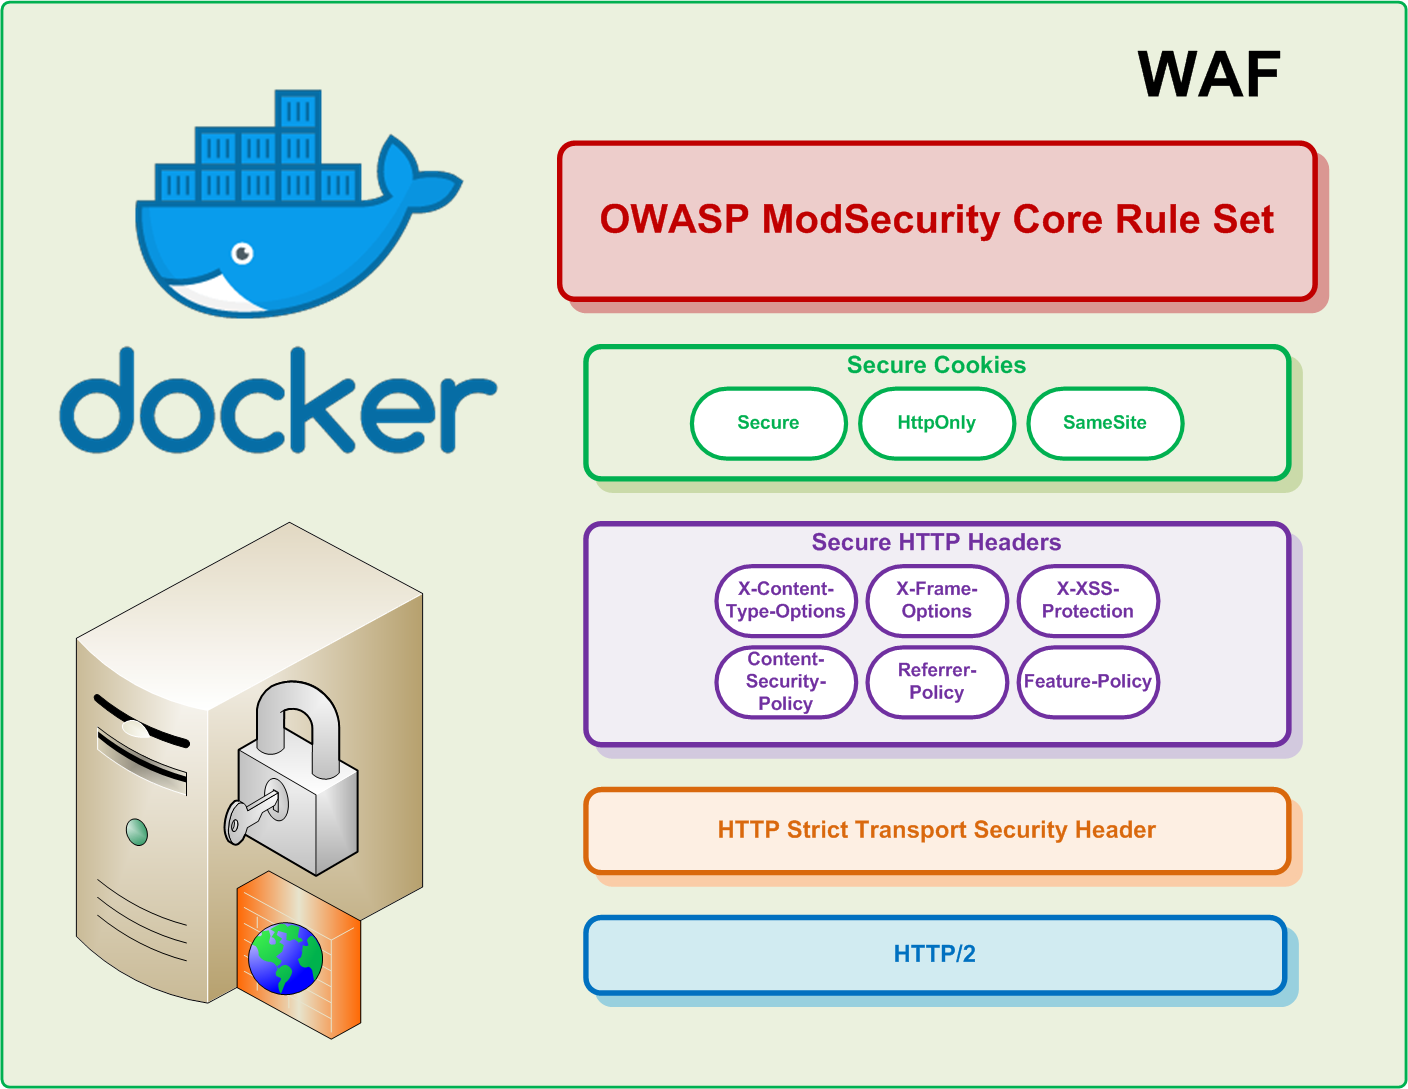
\includegraphics[width=0.7\textwidth]{fig/Diagram_Docker_WAF}
  \caption{Controles de seguridad desplegados en el contenedor Docker.}
\end{figure}

\subsection{Software de gestión de certificados HTTPS}
\par Se ha elegido Let's Encrypt para gestionar los certificados, pues permite que la gestión sea automática y no tiene coste económico.
\par En el \hyperref[fig:Diagram_LetsEncypt_LLD]{diagrama de Let's Encrypt} se puede ver cómo se han definido las comunicaciones entre la instancia de Let's Encrypt desplegada en el cluster de Kubernetes y el servicio SaaS
ofrecido por el proveedor.
\begin{figure}[!ht]
  \centering
  \label{fig:Diagram_LetsEncypt_LLD}
  \includegraphics[width=0.7\textwidth]{fig/Diagram_LetsEncypt_LLD}
  \caption{Diagrama de comunicaciones de Let's Encrypt.}
\end{figure}
\par El modo de funcionamiento es el siguiente:
\begin{enumerate}
  \item La instancia de Docker crea una clave privada.
  \item La instancia de Docker realiza una petición de certificado al servicio SaaS.
  \item El servicio SaaS le comunica una variable temporal no predecible (tipo NONCE) al cliente Let's Encrypt.
  \item La instancia de Docker crea un fichero accesible por el servicio SaaS mediante petición HTTP con el valor propuesto como nombre de fichero.
  \item La instancia de Docker responde al servicio SaaS con el fichero temporal firmado con su clave privada.
  \item El servicio SaaS realiza una petición HTTP para comprobar que la instancia de Docker tiene control sobre el dominio sobre el que se pide el certificado.
    \par La taxonomía de la petición es \lstinline{http://<dominio>:80/.well-known/acme-challenge/<variable-NONCE>}.
  \item El servicio SaaS valida la respuesta HTTP y, a continuación, valida al agente Let's Encrypt.
\end{enumerate}
\par Una vez el agente ha sido autorizado, éste podrá pedir un nuevo certificado, renovarlo o revocarlo.

\subsection{Software de automatización u orquestación}
\par Se ha elegido Kubernetes para gestionar y automatizar la solución.
\par Para ello, se han definido los siguientes elementos:
\begin{itemize}
  \item Para el WAF:
    \begin{itemize}
      \item {\em ccwaf deployment}. Es el componente encargado de desplegar las instancias de WAF.
      \item {\em ccwaf service}. Es el componente encargado de publicar los PODs desplegados y ofrecer abstracción a los servicios externos.
    \end{itemize}
  \item Para el servidor web:
    \begin{itemize}
      \item {\em basicwebserver deployment}. Es el componente encargado de desplegar las instancias de servicio web.
      \item {\em basicwebserver service}. Es el componente encargado de publicar los PODs desplegados.
    \end{itemize}
  \item Para el servidor de Let's Encrypt:
    \begin{itemize}
      \item {\em basicwebserver deployment}. Es el componente encargado de desplegar la instancia de Let's Encrypt.
      \item {\em letsencrypt service}. Es el componente encargado de publicar los PODs desplegados.
    \end{itemize}
\end{itemize}

\par A continuación se muestran los aspectos más representativos de estos elementos:

\subsubsection{ccwaf deployment}
\begin{minipage}{0.8\linewidth}
  \lstinputlisting[language=bash,caption=\lstname,linerange={27-64}]{\codePath/Kubernetes/kub_waf-server.yaml.template}
\end{minipage}
\par Se destacan los siguientes elementos:
\par \lstinline{replicas: 2}. Indica el número de instancias que se despliegan. En las pruebas se han desplegado entre dos y cinco instancias con el fin de validar múltiples instancias en la plataforma.
\par \lstinline{image: <SET_REGISTRY>/<SET_OWNER>/ccwaf:<SET_RELEASE>}. Indica el repositorio desde el que
se descargarán las imágenes. En la elaboración del proyecto se ha utilizado un repositorio propio, pero se
compartirá a un repositorio público tras realizar la entrega.
\par \lstinline{volumeMounts}. Indica el servicio de ficheros que se utilizará para compartir certificados.
Este recurso debe ser inmutable y tolerante a reconstrucciones del entorno, por lo que se ha utilizado un
servicio NFS externo a la plataforma de Kubernetes.

\subsubsection{ccwaf service}
\begin{minipage}{0.8\linewidth}
  \lstinputlisting[language=bash,caption=\lstname,linerange={1-23}]{\codePath/Kubernetes/kub_waf-server.yaml.template}
\end{minipage}
\par En esta configuración destaca el parámetro \lstinline{type: NodePort}, pues el valor {\em NodePort}
indica que el WAF será accesible externamente desde Internet.

\subsubsection{ basicwebserver deployment}
\begin{minipage}{0.8\linewidth}
  \lstinputlisting[language=bash,caption=\lstname,linerange={24-61}]{\codePath/Kubernetes/kub_basicwebserver-server.yaml.template}
\end{minipage}
\par Se puede ver que este elemento es similar al desplegado para el WAF. En esta ocasión se han
desplegado entre dos y cinco instancias en las pruebas con el fin de validar que el entorno distribuido
funciona correctamente.


\subsubsection{ basicwebserver service}
\begin{minipage}{0.8\linewidth}
  \lstinputlisting[language=bash,caption=\lstname,linerange={1-20}]{\codePath/Kubernetes/kub_basicwebserver-server.yaml.template}
\end{minipage}
\par Se puede comprobar como en este servicio se ha configurado el siguiente parámetro: \lstinline{type: ClusterIP}.
\par Al utilizar el valor {\em ClusterIP} se define que las instancias gestionadas por este servicio sólo
son accesibles internamentes al cluster de Kunernetes y, por lo tanto, no son accesibles desde Internet.
\par Con esto se garantiza que las peticiones que se realicen a la plataforma web deben provenir
forzosamente del WAF, con lo que {\bf se garantiza que los mecanismos de protección del WAF serán
aplicados}.

\subsubsection{ basicwebserver deployment}
\begin{minipage}{0.8\linewidth}
  \lstinputlisting[language=bash,caption=\lstname,linerange={24-61}]{\codePath/Kubernetes/kub_basicwebserver-server.yaml.template}
\end{minipage}
\par En esta ocasión se ha desplegado una única réplica, pues este servicio está dedicado a la gestión de
certificados, un servicio al que los usuarios no tienen acceso y con un consumo menor de recursos.

\subsubsection{ letsencrypt service}
\begin{minipage}{0.8\linewidth}
  \lstinputlisting[language=bash,caption=\lstname,linerange={1-20}]{\codePath/Kubernetes/kub_basicwebserver-server.yaml.template}
\end{minipage}
\par Al igual que en el servicio web, se ha optado por proteger el servicio Let's Encrypt con el WAF, por
lo que se ha definido nuevamente \lstinline{type: ClusterIP}.


\subsection{Diseño final}
\par Tras construir todos los componentes necesarios, las peticiones HTTP y HTTPS son tal como se indica en el \hyperref[fig:Diagram_HTTP_Services]{Diagrama de peticiones HTTP/HTTPS en la solución}.
\begin{figure}[!ht]
  \centering
  \label{fig:Diagram_HTTP_Services}
  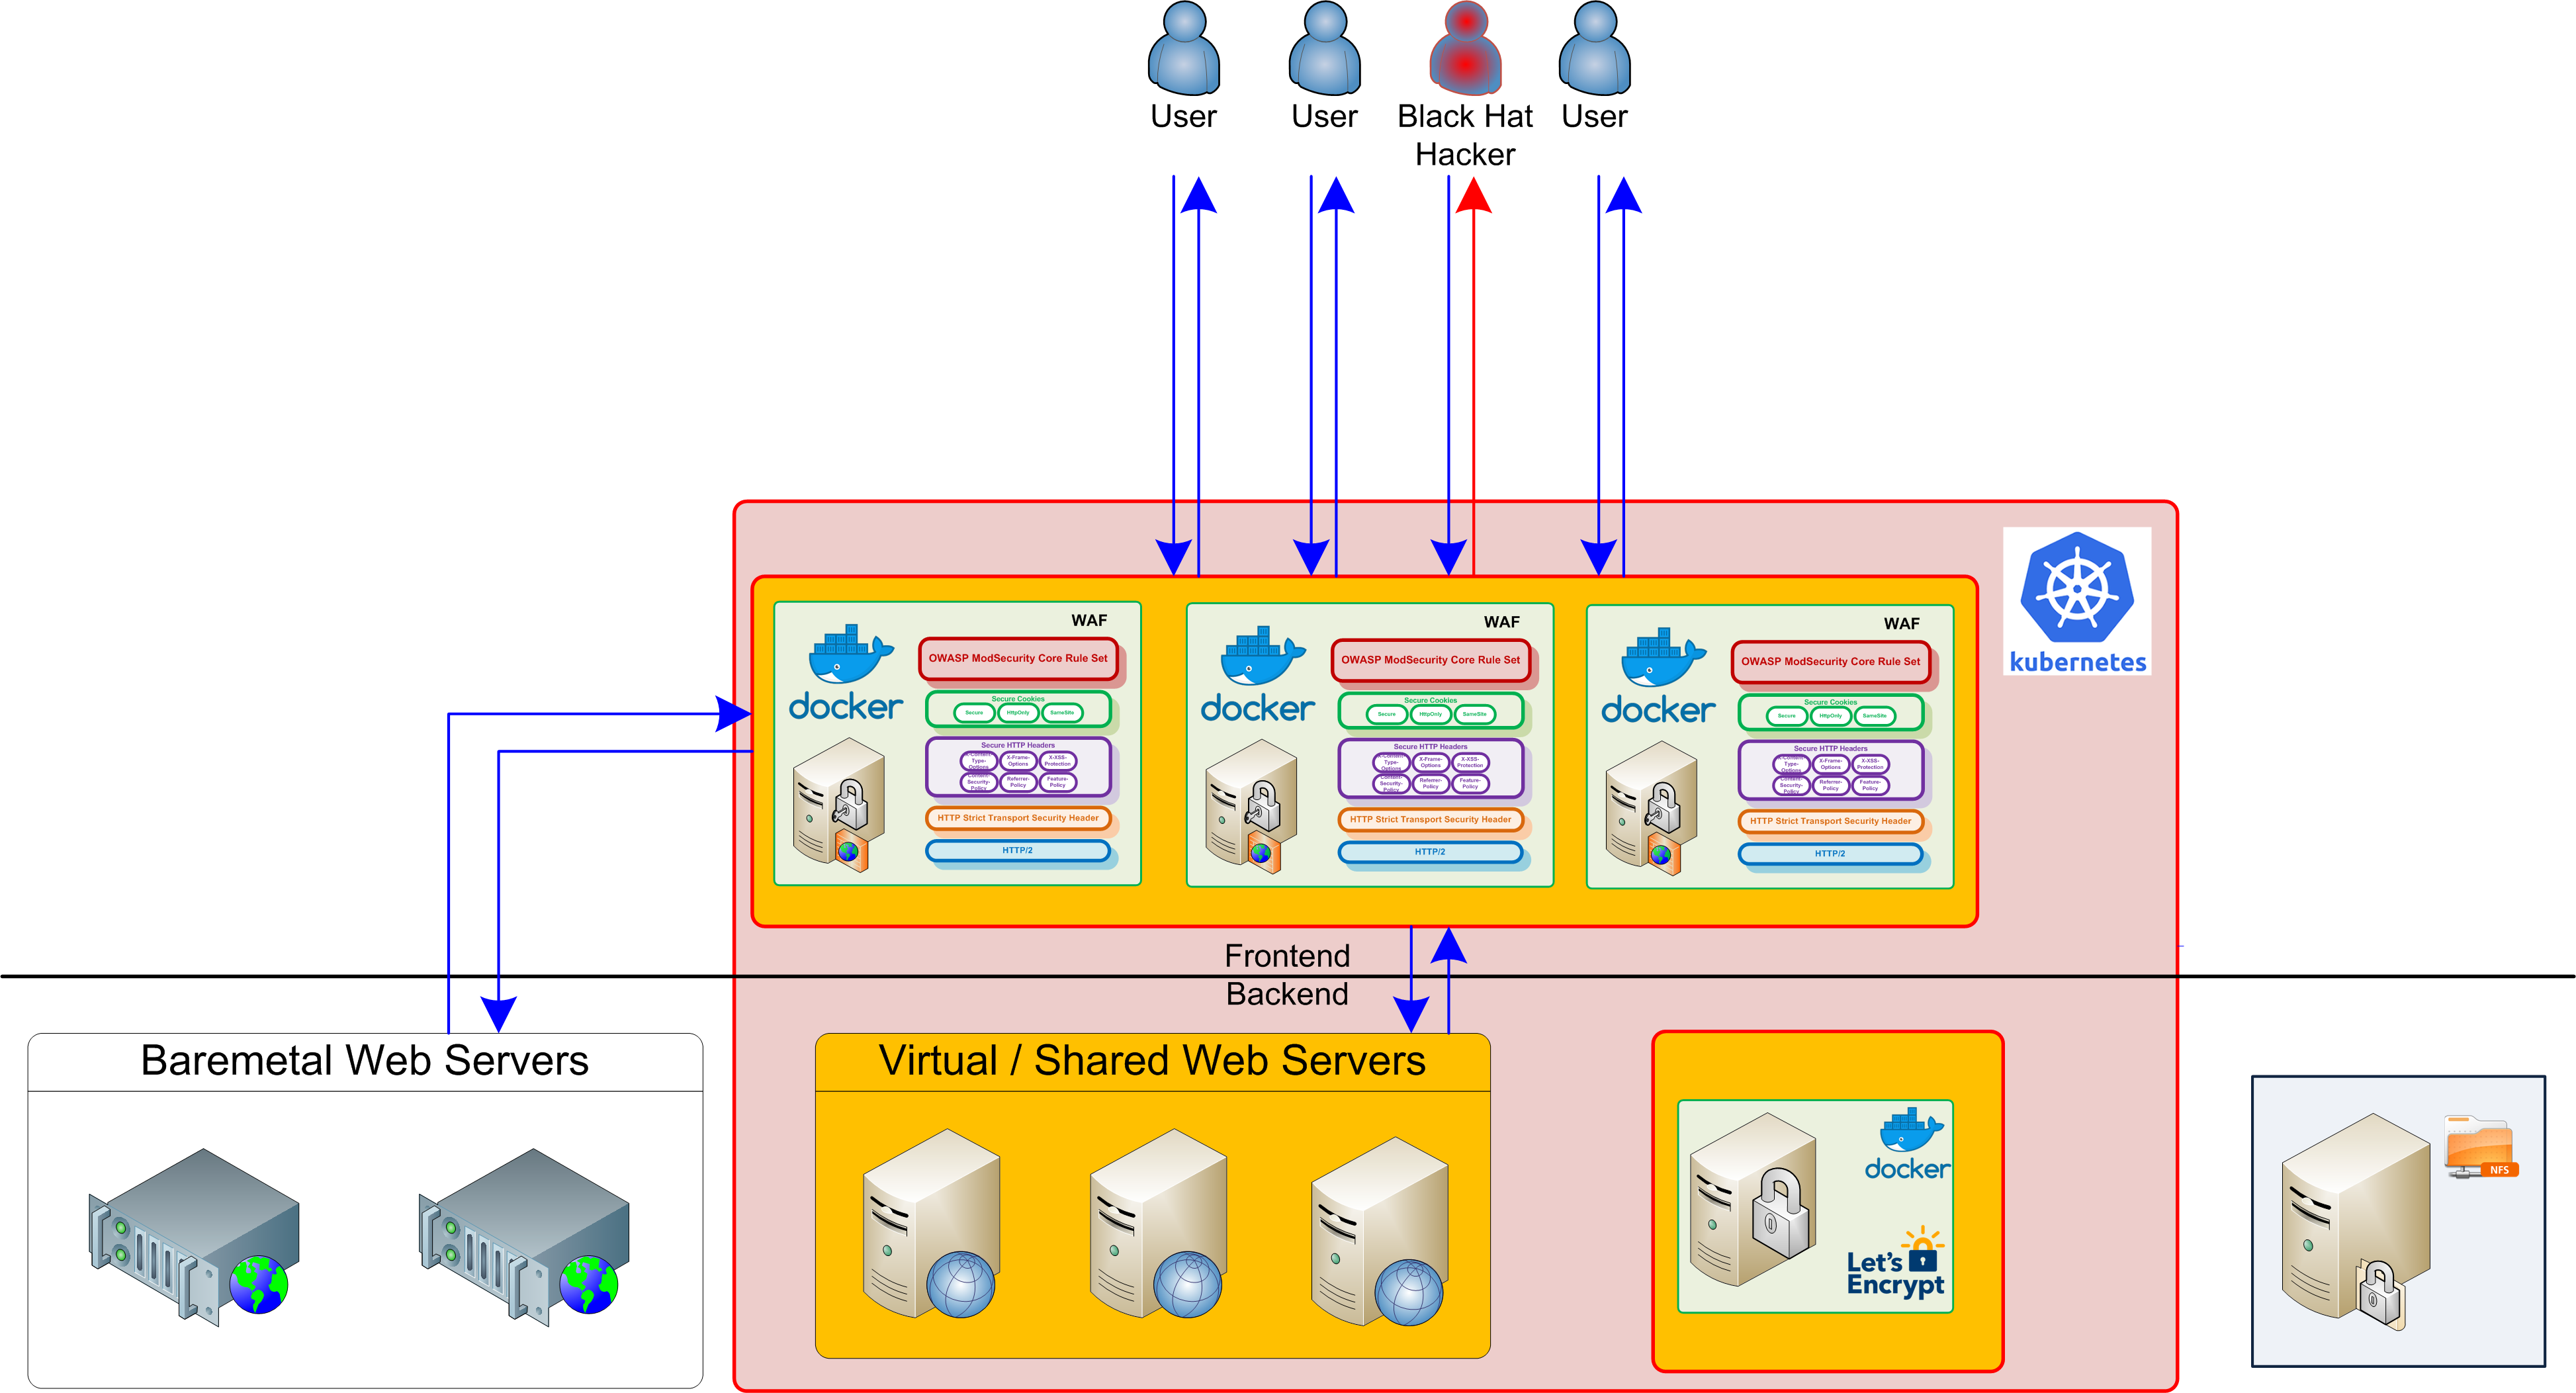
\includegraphics[width=\textwidth]{fig/Diagram_HTTP_Services}
  \caption{Diagrama de peticiones HTTP y HTTPS}
\end{figure}


\section{Viabilidad Económica}
\par Una de los principales motivos por los que las soluciones WAF no son más frecuentes, es su elevado coste, tal como se ha detallado en la sección de ~\nameref{subsec:estadoarte}.
\par Es por ello que se ha priorizado utilizar tecnologías sin coste de licenciamiento y minimizar otros costes lo máximo posible.
\par No obstante, la solución tiene una serie de costes que se deben considerar:
\begin{itemize}
  \item Plataforma hardware o de Cloud sobre la que se desplegará la solución.
  \item Horas de técnico administrador de la plataforma.
  \item Soporte técnico del proveedor. Opcional.
\end{itemize}

\par Estos costes pueden variar considerablemente dependiendo de la plataforma sobre la que se despliegue la solución.
\par La opción más económica será aquella en la que la plataforma hardware y los técnicos disponibles pueden asumir la carga adicional que la solución requiere; en este escenario sólo se deberá contemplar el coste del
soporte técnico, el cual es así mismo opcional. Por lo tanto en este escenario la solución no tendría un {\bf coste económico directo}.

\par Otro posible escenario, consistiría en desplegar la solución en algún proveedor del Cloud. Esta arquitectura es cada vez más frecuente y es importante evaluar su coste.
\par En primer lugar se debe estimar el coste de la plataforma en sí. Para ello se ha utilizado la herramienta online proporcionada por Azure~\cite{azurecalculator}.


\begin{figure}[!ht]
  \centering
  \begin{tabular}{|p{0.15\textwidth}|p{0.13\textwidth}|p{0.35\textwidth}|p{0.2\textwidth}|}
  \hline
  {\bf Service type}              & {\bf Region}  & {\bf Description}                                                                           & {\bf Estimated Cost}                \\
  \hline
  Azure Kubernetes Service (AKS)  & West Europe   & 5 D2 v3 (2 vCPU(s), 8 GB RAM) nodes x 730 Hours; Pay as you go; 1 managed OS disks – S4     & 370.66€                             \\
  \hline
  Storage Accounts                & West Europe   & File Storage, Standard Performance Tier, General Purpose V2, LRS Redundancy, 100 GB \
                          Capacity, 1 Put or Create Container operations, 1 List operations, 1 Other operations, 0 Additional Sync servers      & 5.09€                               \\
  \hline
  Container Registry              & West Europe   & Basic Tier, 1 units x 30 days, 100 GB Bandwidth                                             & 11.18€                              \\
  \hline
  Support                         &               & Support                                                                                     & 0.00€                               \\
  \hline
                                  &               & Licensing Program                                                                           & Microsoft Online Services Agreement \\
  \hline
                                  &               & Monthly Total                                                                               & 386.93€                             \\
  \hline
                                  &               & Annual Total                                                                                & 4643.18€                            \\
  \hline
  \end{tabular}
  \label{tabla:azurecalculatoraks}
  \caption{Estimación económica de la plataforma de contenedores en Microsoft Azure AKS~\cite{aks} (fuente~\cite{azurecalculator})}
\end{figure}

\par A este coste hay que añadir el tiempo en horas del administrador de la plataforma. Según la misma plataforma de Azure, esta plataforma requiere una media de 15.5 horas anuales con un coste de 50€/hora. Lo que nos da
la siguiente estimación:

\begin{figure}[!ht]
  \centering
  \begin{tabular}{|p{0.3\textwidth}|p{0.15\textwidth}|p{0.15\textwidth}|p{0.2\textwidth}|}
  \hline
  {\bf Recurso}               & {\bf Tiempo}  & {\bf Coste/hora}    & {\bf Coste Total}           \\
  \hline
    Administrador DevOps      & 15.5 horas  & 50€                 & 775€ \\
  \hline
                              &             & Total anual         & 775€ \\
  \hline
  \end{tabular}
  \label{tabla:azurecalculatorsalary}
  \caption{Estimación económica de Microsoft Azure (fuente~\cite{azurecalculator})}
\end{figure}

\par Por último, para calcular el coste de soporte técnico, dado que la solución está compuesta de múltiples tecnologías, no se considera viable añadir el coste del soporte técnico de todas ellas.
\par A modo de referencia se ha evaluado el coste del soporte 24/7 de Nginx para cuatro instancias y el coste es el siguiente:

\begin{figure}[!ht]
  \centering
  \begin{tabular}{| c | c | c | c |}
  \hline
  {\bf Tipo de soporte}           & {\bf Número de instancias}    & {\bf Coste/instancia}   & {\bf Coste Total}   \\
  \hline
    Professional (soporte 24/7)   & 4                             & 3109.02 / año           & 12436.06€           \\
  \hline
                                  &                               & Total anual             & 12436.06€           \\
  \hline
  \end{tabular}
  \label{tabla:nginxplus}
  \caption{Coste del soporte técnico de Nginx (fuente~\cite{nginxplus})}
\end{figure}

\par Se pueden ver los costes consolidados en la \hyperref[tabla:costesresumen]{Tabla resumen de la viabilidad económica} \\

\begin{figure}[!ht]
  \centering
  \begin{tabular}{| p{0.3\textwidth} | c | c | c | c |}
  \hline
    {\bf Entorno}                                             & {\bf Plataforma}  & {\bf Administración}  & {\bf Soporte} & {\bf Coste total}   \\
  \hline
    Entorno Cloud con soporte Nginx                           & 4643€                   & 775€                        & 12436.06 €           & 17854.06 €         \\
  \hline
    Entorno Cloud sin soporte Nginx                           & 4643€                   & 775€                        & 0 €                  & 5418 €             \\
  \hline
    Entorno on-premise sin HW adicional con soporte Nginx  & 0€                      & 775€                        & 12436.06 €           & 13211.06 €         \\
  \hline
    Entorno on-premise sin HW adicional sin soporte Nginx  & 0€                      & 775€                        & 0 €                  & 775 €              \\
  \hline
  \end{tabular}
  \label{tabla:costesresumen}
  \caption{Resumen de costes estimados}
\end{figure}

\par Es importante reseñar que se ha considerado el soporte Nginx como un caso representativo del elevado coste que tienen este tipo de servicios. Habitualmente no es necesario
contratar este tipo de soluciones en entornos que no sean críticos o muy sensibles y, en estos entornos se requiere un soporte equivalente de todos los componentes.
\par En los entornos en los que no se requiere un servicio de este tipo, es habitual optar por servicios profesionales y de consultoría, sea bajo demanda o con la contratación de
una bolsa de horas.


\chapter {Resultados}
\par En esta sección se exponen los aspectos más destacados de la solución construida.

\section{Facilidad de despliegue}
\par La solución es fácilmente desplegable en entornos Kubernetes. Para ello, sólo será necesario realizar los siguientes pasos:
\begin{enumerate}
  \item Descargar repositorio: \\
		\begin{minipage}{\linewidth}
		\begin{lstlisting}[language=bash]
git clone git@github.com:bpk667/CircumCaetera.git
		\end{lstlisting}
		\end{minipage}
  \item Definir parámetros del entorno. \\
		\begin{minipage}{\linewidth}
		\begin{lstlisting}[language=bash]
DOMAIN="example.org"                          # Domain for the web services.
OWNER="$(whoami)"                             # Ownner of the Docker registry.
EMAIL="example@protonmail.com"                # Required by Let's Encrypt.
CERTIFICATEPATH="/exports/certs/${DOMAIN}"    # Host NFS repository for sharing certificates.
REGISTRY="localhost:5000"                     # Docker registry.
NFSSERVER="NFS_SERVER_IP"                     # IP of the NFS server
		\end{lstlisting}
		\end{minipage}
  \item Desplegar la aplicación. \\
		\begin{minipage}{\linewidth}
		\begin{lstlisting}[language=bash]
CircumCaetera/scripts/cc_deployWAF.sh
		\end{lstlisting}
		\end{minipage}
\end{enumerate}

No obstante, este despliegue tiene como requisitos que los registros DNS y el recurso NFS hayan sido previamente configurados.

\section{Adaptabilidad de la solución}
\par Dado que todo el proyecto está licenciado con licencia \acrlong{gpl} versión 3, cualquier que necesite modificar la solución puede hacerlo.
\par Por otro lado, toda la solución ha sido diseñada de forma modular con el fin de facilitar su uso parcial en los entornos en los que así se requiera. Algunos ejemplos de casos de uso en los que se utilice algún componente de la solución: 
\begin{itemize}
\item Se requiere implementar TLS adecuadamente, pero no se quieren utilizar los componentes WAF.
\item Se quiere desplegar WAF+TLS en un entorno Docker con un orquestador diferente.
\item Se quiere desplegar la solución WAF+TLS sin el gestor de certificados debido a que se dispone de una CA propia.
\end{itemize}

\section{Controles adicionales}
\par Se han implementado una serie de controles adicionales que no son estrictamente competencia de un WAF, como son la mejora de en la seguridad de las cookies, las cabeceras de seguridad o forzar el uso de canales
cifrados mediante la cabecera \cite{wiki:hsts}.
\par Adicionalmente, se ha configurado un gestor de certificados que permite implementar HTTPS de forma sencilla para el usuario.

\section{Validación de la seguridad}
Para poder validar la seguridad ofrecida por la solución, se ha escaneado la plataforma con las siguientes herramientas:
\par {\em Qualys. SSL Labs~\cite{ssllabs}}. Se trata de una herramienta online que ejecuta una batería de pruebas con el objetivo de verificar la seguridad de la página web.
\par En la figura ~\hyperref[tabla:resumenqualys]{Resumen ejecutivo de Qualys SSL Labs} se puede ver un resumen del resultado de las pruebas. En el apéndice
(~\hyperref[tabla:informequalys]{Informe completo de Qualys} ) se puede leer el informe completo.

\begin{figure}[!ht]
  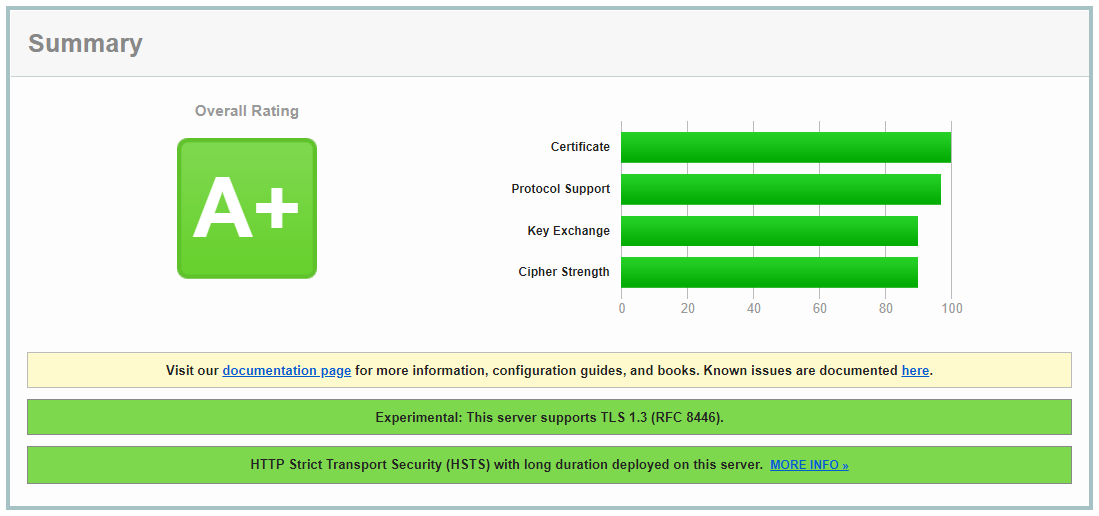
\includegraphics[width=0.9\textwidth]{fig/SSLTLS_Report_Summary}
  \label{tabla:resumenqualys}
  \caption{Resumen ejecutivo de Qualys SSL Labs}
\end{figure}
\par Entre otros, los test ejecutados incluyen: Configuración TLS, vulnerabilidades TLS y configuración de certificados.

\par Otra herramienta online que se ha ejecutado es {\em Security Headers} de Netsparker~\cite{securityheaders}.
\par En la figura ~\hyperref[tabla:resumensecurityheaders]{Resumen ejecutivo de Security Headers} se puede ver un resumen del resultado de las pruebas. En el apéndice
(~\hyperref[tabla:informesecurityheaders]{Informe completo de Security Headers} ) se puede leer el informe completo.

\begin{figure}[!ht]
  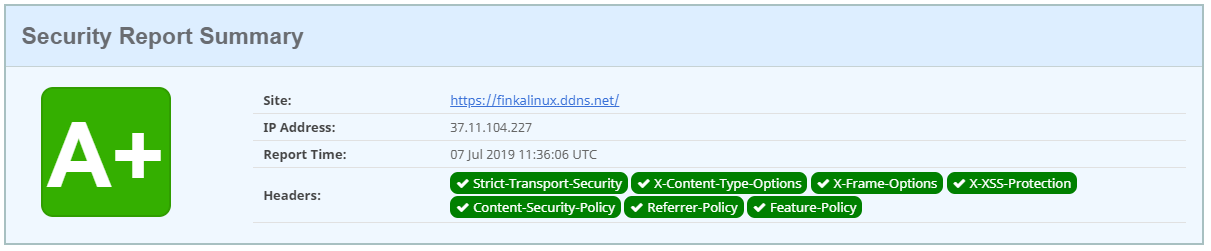
\includegraphics[width=0.9\textwidth]{fig/SecurityHeaders_Report_Summary}
  \label{tabla:resumensecurityheaders}
  \caption{Resultados cabeceras HTTP de seguridad}
\end{figure}
Entre otros, los test ejecutados incluyen: {\em \acrlong{hsts}} (\acrshort{hsts}), {\em X-XSS-Protection}, {\em Content-Security-Policy} o la reciente {\em Feature-Policy}.



\section{Conclusiones}
\begin{frame}[shrink]
  \frametitle{Conclusiones}
  TODO
\end{frame}




% Print glossary
\printglossary[title=Acrónimos,type=\acronymtype]
\printglossary[title=Glosario]
 
% Print bibliography
\printbibliography[heading=bibintoc]


\begin{comment}
  \clearpage
  \appendixpage
  \begin{appendices}
  \end{appendices}
\end{comment}

\clearpage
\appendixpage
\begin{appendices}

\appendix
\chapter{Contrucción de WAF en Docker}
\label{listing:ccwafDockerfile}
\lstinputlisting[language=bash,caption=\lstname,title=\lstname]{\codePath/Docker/ccwaf/Dockerfile.template}
\label{listing:nginx.conf}
\lstinputlisting[language=bash,caption=\lstname,title=\lstname]{\codePath/Docker/ccwaf/files/nginx_conf/nginx.conf}
\label{listing:default.conf}
\lstinputlisting[language=bash,caption=\lstname,title=\lstname]{\codePath/Docker/ccwaf/files/nginx_conf/sites-available/default.conf.template}
\label{listing:hide_headers.conf}
\lstinputlisting[language=bash,caption=\lstname,title=\lstname]{\codePath/Docker/ccwaf/files/nginx_conf/snippets/hide_headers.conf}
\label{listing:proxy_headers.conf}
\lstinputlisting[language=bash,caption=\lstname,title=\lstname]{\codePath/Docker/ccwaf/files/nginx_conf/snippets/proxy_headers.conf}
\label{listing:security_headers.conf}
\lstinputlisting[language=bash,caption=\lstname,title=\lstname]{\codePath/Docker/ccwaf/files/nginx_conf/snippets/security_headers.conf}


\end{appendices}



\end{document}
